\documentclass[10pt,TimesNewRoman,a4paper]{matrikenglish}
\setlength{\headsep}{0.3in}
\usepackage{amsmath, amsfonts, amssymb, float, fancyhdr}
\usepackage[figuresright]{rotating}
\usepackage{authblk, graphicx, indentfirst, lastpage, lipsum}
\usepackage{pifont}
\renewcommand{\Authsep}{, }
\renewcommand{\Authand}{, }
\renewcommand{\Authands}{, }
\setlength{\affilsep}{0cm}
\renewcommand\Authfont{\normalsize}
\renewcommand\Affilfont{\normalfont\small}
\makeatletter
\renewcommand{\@biblabel}[1]{[#1]\hfill}
\makeatother
\usepackage{subfig, caption, epstopdf}
\usepackage[left=1.2cm, right=1.2cm, top=2.2cm, bottom=3.3cm, includeheadfoot]{geometry}% atas bawah 2.5 kanan kiri 1.5
\usepackage[justification=centering]{caption}
\captionsetup{labelsep=period}
\usepackage{titlesec}
\usepackage{xcolor}
\usepackage[x11names]{xcolor}
\titleformat{\section}
{\normalfont\normalsize\bfseries\uppercase}{\thesection}{1.7em}{}
\titleformat{\subsection}
{\normalfont\normalsize\bfseries}{\thesubsection}{.95em}{}
\titleformat{\subsubsection}{\bfseries}{\thesubsubsection}{.95em}{}
\titlespacing*{\section}{0cm}{0.7cm}{0.1cm}
\titlespacing*{\subsection}{0cm}{0.7cm}{0.1cm}
\titlespacing*{\subsubsection}{0.8cm}{0.7cm}{0.1cm}
\usepackage{enumitem}
\usepackage[numbers,compress]{natbib}
\usepackage[hidelinks]{hyperref}
\hypersetup{
	colorlinks   = true, 
	urlcolor     = blue, 
	linkcolor    = blue, 
	citecolor    = blue  
}
\setlist{nolistsep}
\usepackage{multirow}
\CopyrightLine[]{Copyright \textcopyright2022 The Authors.\\}{This is an open access article under the \href{https://creativecommons.org/licenses/by-sa/4.0/}{\textcolor{blue}{\underline{CC BY-SA}}} license.}
\vspace{.5em}

%%---------------------------------------------------------------------
%% MULAI ISI DISINI

%% isi nama penulis
\author[1]{\bfseries Leonardo Alfontus Mende Sirait}
\author[2]{\bfseries Martin Clinton Tosima Manullang, Ph.D.}
\author[3]{\bfseries Leslie Anggraini, S.Kom., M.Cs.}

%%isi afiliasi penulis
\affil[1]{Institut Teknologi Sumatera, South Lampung, Indonesia}
\affil[2]{Second Affiliation, City, Country}

%%isi judul dan judul pendek (untuk di footer)
\title{\vspace{.3in}Development of Fall Position Detection in the Elderly Using a Pose Landmark-Based Graph Convolutional Network}
\shorttitle{Development of Fall Position Detection in the Elderly Using a Pose Landmark-Based Graph Convolutional Network}

%%starting
\begin{document}
\setcounter{page}{1} %% isi halaman awal jurnal

%%indentation. do not change
\setlength{\parindent}{.9cm}

%%header and footer setting. do not change
\pagestyle{fancy}
\fancyhfoffset{0cm}

%%journal info
\journalname{Matrik: Jurnal Manajemen, Teknik Informatika, dan Rekayasa Komputer}
\journalshortname{Matrik: Jurnal Managemen,Teknik Informatika, dan Rekayasa Komputer}
\journalhomepage{\href{https://journal.universitasbumigora.ac.id/index.php/matrik}{https://journal.universitasbumigora.ac.id/index.php/matrik}}
\vol{xx} %isi volume
\no{x} %isi nomor
\months{Bulan} %isi bulan
\years{Tahun} %isi tahun
\issn{2476-9843, \href{accredited by Kemenristekdikti, Decree No: 200/M/KPT/2020}{\underline{accredited by Kemenristekdikti, Decree No: 200/M/KPT/2020}}} %isi ISSN yg sesuai
\issnshortname{2476-9843} %ISSN untuk header halaman isi
\DOI{10.30812/matrik.vxxix.xxx} %isi DOI yg sesuai
\pagefirst{xx} %isi halaman awal
\pagelast{xx} %isi halaman akhir

%%build title
\maketitle

%%border setting. do not change
\hrule
\vspace{.1em}
\hrule
\vspace{.5em}
\noindent
\parbox[t][][s]{0.275\textwidth}{%
\textbf{Article Info}
\vspace{.5em}
\hrule
\vspace{.5em}
\begin{history}
\vspace{.5em}

%%informasi artikel dan privilege editor
%isi tanggal yang sesuai
Received mm dd, yyyy

Revised mm dd, yyyy

Accepted mm dd, yyyy

\vspace{.7em}
\end{history}
\vspace{.5em}
\hrule
\vspace{.5em}
\begin{keyword} 
	\vspace{.5em}
	%%isi keywords disini, dipisahkan dengan \sep
	Graph Convolutional Network \sep Mediapipe \sep Eldery \sep Fall \sep Deep Learning \sep Pose Landmark \sep Ablation Study
	\vspace{.5em}
\end{keyword}
\vspace{\fill}
}
\parbox{0.025\textwidth}{\hspace{0.5em}}
\parbox[t][][s]{0.69\textwidth}{%
\begin{abstract}
	\vspace{.3em}
	%%isi abstract disini
	Falls among older adults were identified as a major health problem because they often caused injury, repeated incidents, and reduced quality of life, especially among nursing home residents. This study developed a fall-position detection model that could operate continuously in less supervised environments. Unlike earlier image-based approaches that required high computational power, this study used pose landmark data to build a model based on graph convolutional networks, which was technically lighter and more efficient. Two hyperparameter settings were tested, consisting of a default configuration and a configuration derived from an ablation study. The results showed that the ablation-based configuration performed better than the default configuration across all evaluation measures. On average, accuracy increased by 0.018, precision by 0.024, F1-score by 0.049, and recall by 0.093, with recall showing the largest improvement. These findings indicated that the optimized model improved fall detection performance and showed strong potential for future elderly health monitoring systems focused on distinguishing fall and non-fall events.
\end{abstract}
}
\parbox[l]{\textwidth}


\noindent
	\parbox[l]{\textwidth}{%
	\rule{\textwidth}{0.5pt}
	\\
	\emph{\textbf{Corresponding Author:}}
	\vspace{.5em}\\
	%% isi informasi tentang korespondensi, dipisahkan dengan \\
	Name of Corresponding Author, HP\\
	Faculty and Study Program,\\
	Affiliation, City, Country,\\
	Email: {\href{mailto:corresp-author@xxxxxxxx}{corresp-author@xxxxxxxx}}\\
	
}
\hrule
\vspace{.1em}
\hrule
\vspace{1cm}
\noindent
How to Cite:\\
%P.M. Morse and H.Feshback, "Methods of Theoretical Physic". New York: McGraw Hill, 1953.\\
This is an open access article under the CC BY-SA license (\href{https://creativecommons.org/licenses/by-sa/4.0/}{\underline{https://creativecommons.org/licenses/by-sa/4.0/}})

\newpage
%%----------------------------------------------------------------------
% mulai bagian isi jurnal

\section{INTRODUCTION}
\label{}

Older adults represent a growing segment of the global population, and aging is a natural stage of the human life cycle experienced by every individual. The World Health Organization classifies people aged 60 years and above as older adults \cite{Gusti2023}. As age increases, physical and health-related functions tend to decline progressively. Physiological changes such as reduced muscle mass, decreased bone density, and impaired balance make older adults more vulnerable to health and safety problems, including falls \cite{Colon2018}.

A fall can be understood as an event in which a person unexpectedly comes to rest on the ground, floor, bed, or another lower surface, either unintentionally or due to loss of postural control, often resulting in injury \cite{Forrest2012}. Older adults are particularly susceptible to fall-related injuries because of sensory decline, balance disorders, muscle weakness, and the side effects of medication \cite{Colon2024}. According to global health statistics, approximately 37.3 million falls require medical attention each year, and around 684,000 deaths worldwide are associated with falls \cite{Who2021}. The burden is even greater in institutional care settings. Older adults living in nursing homes experience falls more frequently than those living at home, with an annual incidence of 30\% to 50\%, and about 40\% of them experiencing recurrent falls \cite{ACEBAC2023}. In Indonesia, the incidence of falls among older adults aged 65 years and above is reported to be around 30\%, increasing to approximately 50\% among those aged over 80 years \cite{Gusti2023}.

The risk becomes more serious in nursing homes and other long-term care environments, where older adults may spend periods of time without direct supervision. Previous research showed that fall rates in long-term care facilities were substantially higher than in private or family settings, with an average of nearly two falls per resident per year \cite{Albasha2024}. Falls also tend to occur more frequently at night or during staff shift changes, when supervision is reduced \cite{Albasha2024}. This condition creates a critical need for an effective early warning system that can detect falls promptly in locations where continuous observation is not always possible.

Delayed assistance after a fall may lead to severe complications and even death. Reduced muscle function after falling often prevents older adults from standing up independently. Remaining on the floor for more than one hour may cause dehydration, hypotension, pneumonia, and pressure ulcers \cite{Fleming2008}. Prolonged lying after a fall has also been associated with increased transition to long-term care \cite{Fleming2008}. Therefore, a fall detection system that operates continuously for 24 hours is essential, especially in environments where caregivers cannot maintain constant visual supervision.

In general, the main challenge is how to provide immediate alerts to caregivers or medical personnel when an older adult experiences a fall. Existing fall detection technologies have been developed through three major approaches: wearable sensors, vision-based systems, and hybrid methods. Wearable approaches, such as accelerometers and inertial measurement units, can capture movement data effectively during daily activities and fall events. However, these systems also have important limitations. Devices attached to the body must be comfortable enough for daily use; otherwise, users may be reluctant to wear them. In addition, wearable devices often require calibration and have limited battery life, which creates the risk of missing a fall event when the device is not functioning properly \cite{Mubashir2013}.

Because of these limitations, computer vision has emerged as a promising alternative. Computer vision enables a system to acquire, process, and interpret information from images or video automatically \cite{Negoro2023}. In fall detection, this approach offers the advantage of non-contact monitoring, which is more suitable for older adults who may not consistently use wearable devices. Recent progress in deep learning has further improved the capability of vision-based systems to recognize human posture and motion patterns. Deep learning uses artificial neural networks with multiple processing layers to extract meaningful representations from data and has been successfully applied in speech recognition, object recognition, and many biomedical applications \cite{LeCun2015}.

Several deep learning-based fall detection systems have been proposed, including models that combine convolutional neural networks and long short-term memory networks to capture spatial and temporal information from image sequences \cite{Chhetri2021}. Although such methods are effective, they usually require high computational resources because they process full image frames. This requirement becomes a significant limitation for practical deployment on low-power devices or in large-scale monitoring systems \cite{Chhetri2021}. Thus, there remains a need for a fall detection approach that is both accurate and computationally efficient.

Pose landmark extraction offers a more efficient alternative to full-frame image processing. MediaPipe, an open-source framework developed for human pose estimation, extracts body keypoints from images or video using deep learning models \cite{Lugaresi2019}. Instead of preserving the entire image, this approach represents the human body through a set of keypoint coordinates, resulting in much smaller and more structured data \cite{Lugaresi2019}. Recent studies reported that optimized pose estimation architectures could reduce frame processing time while improving pose estimation accuracy \cite{Sengar2024}. Pose-based representations also show greater robustness to illumination changes and partial occlusion because they prioritize the detection of body keypoints rather than pixel-level appearance \cite{Raj2024}.

Graph Convolutional Networks (GCNs) provide a suitable method for processing pose landmark data because the human skeleton can naturally be represented as a graph, where joints are treated as nodes and bones as edges. GCNs were introduced as a deep learning method for learning from graph-structured data by exploiting both node features and graph topology \cite{Kipf2016}. In the context of fall detection, this capability makes them well suited for modeling spatial relationships among body joints and capturing posture patterns associated with falling \cite{Zahan2025}. Previous studies demonstrated that GCN-based approaches using pose landmarks could achieve high accuracy and outperform several conventional methods in fall detection tasks \cite{Zhang2023}.

Based on this background, this study focused on the development of a fall detection model using a Graph Convolutional Network based on pose landmark data. The proposed approach aimed to reduce computational complexity compared with conventional image-based deep learning models while preserving important spatial information about body posture. The novelty of this research lies in the application of a graph-based learning framework to lightweight pose representations for continuous fall monitoring in older adults. This approach is expected to support the development of a more efficient and practical early warning system for caregivers and medical personnel, thereby reducing the risk of severe complications and delayed treatment after falls in nursing homes, hospitals, and home-care environments.


\section{RESEARCH METHOD}
\label{}

The overall research process is illustrated in the following flowchart.\par

\begin{figure}[H]
    \centering
    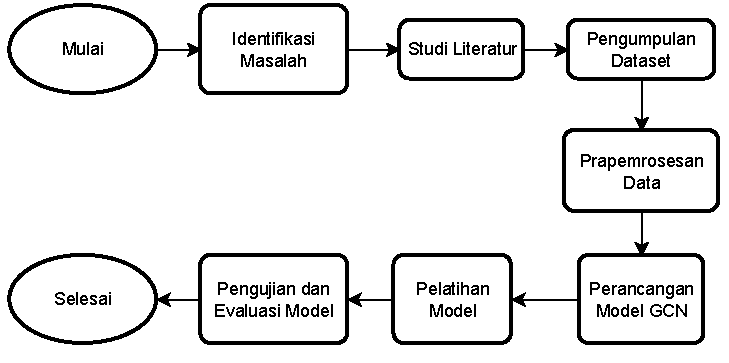
\includegraphics[width=0.55\textwidth]{figure/BAB 3/alur penelitian.pdf}
    \caption{Research flow}
    \label{fig:alur penelitian}
\end{figure}

The stages carried out in this study are presented in Figure \ref{fig:alur penelitian}. The process begins with problem identification and the formulation of research objectives to determine the focus and direction of the study. Next, a literature review is conducted to understand previous relevant studies, broaden insight, and identify limitations or areas that can still be improved in this field. After that, dataset collection is carried out by gathering the video dataset required for the experiments. \par

The next stage is data preprocessing and feature extraction, in which the collected data are processed and prepared for use in the model. This stage includes frame extraction and pose landmark data processing. Subsequently, the GCN model is designed and constructed for use in this study. The model is then trained using the processed dataset, followed by performance evaluation to measure the model's accuracy and effectiveness in detecting fall positions in older adults. This process is iterative, with the model being continuously refined based on the evaluation results. Finally, the study concludes after all stages have been completed. \par

\subsection{Problem Identification} \label{III.identifikasi masalah}

The first stage of this research is the initiation of the overall process, which includes a thorough understanding of the study objectives and the arrangement of the steps to be undertaken. This study begins by defining the general scope and objectives of the research. The main problem addressed is the high number of accidents experienced by older adults, particularly falls that often receive insufficient attention. Falls among older adults frequently result in serious injuries and may even lead to death. \par

Based on this problem, the study focuses on developing a fall-position detection model that can help identify fall events quickly and therefore has the potential to save lives. Accordingly, the objective of this study is to design and build a model capable of analyzing body pose landmark data of older adults using Mediapipe and then utilizing GCN technology to detect fall positions based on these data. \par

\subsection{Literature Review} \label{III.studi literatur}

This step can be considered the main foundation of the study. The following stages in the research flow require substantial knowledge that can be obtained from various sources, one of which is research literature. Previous studies related to this research topic were reviewed using keywords such as Graph Convolutional Network (GCN), fall events in older adults, Mediapipe, pose landmark, and related terms. \par

\subsection{Dataset Collection} \label{III.pengumpulan data}

The next step is the collection of the dataset required for this research. A dataset\footnote{https://iiw.kuleuven.be/onderzoek/advise/datasets\#High\%20Quality\%20Fall\%20Simulation\%20Data} provided in the paper entitled "Bridging the gap between real-life data and simulated data by providing realistic fall dataset for evaluating camera-based fall detection algorithms" was used. This dataset consists of body-movement videos captured using a 2-dimensional camera. The dataset was developed to document various scenarios in a realistic environment. Different fall scenarios were designed to imitate actual fall incidents as accurately as possible. \par

\begin{figure}[H]
    \centering
    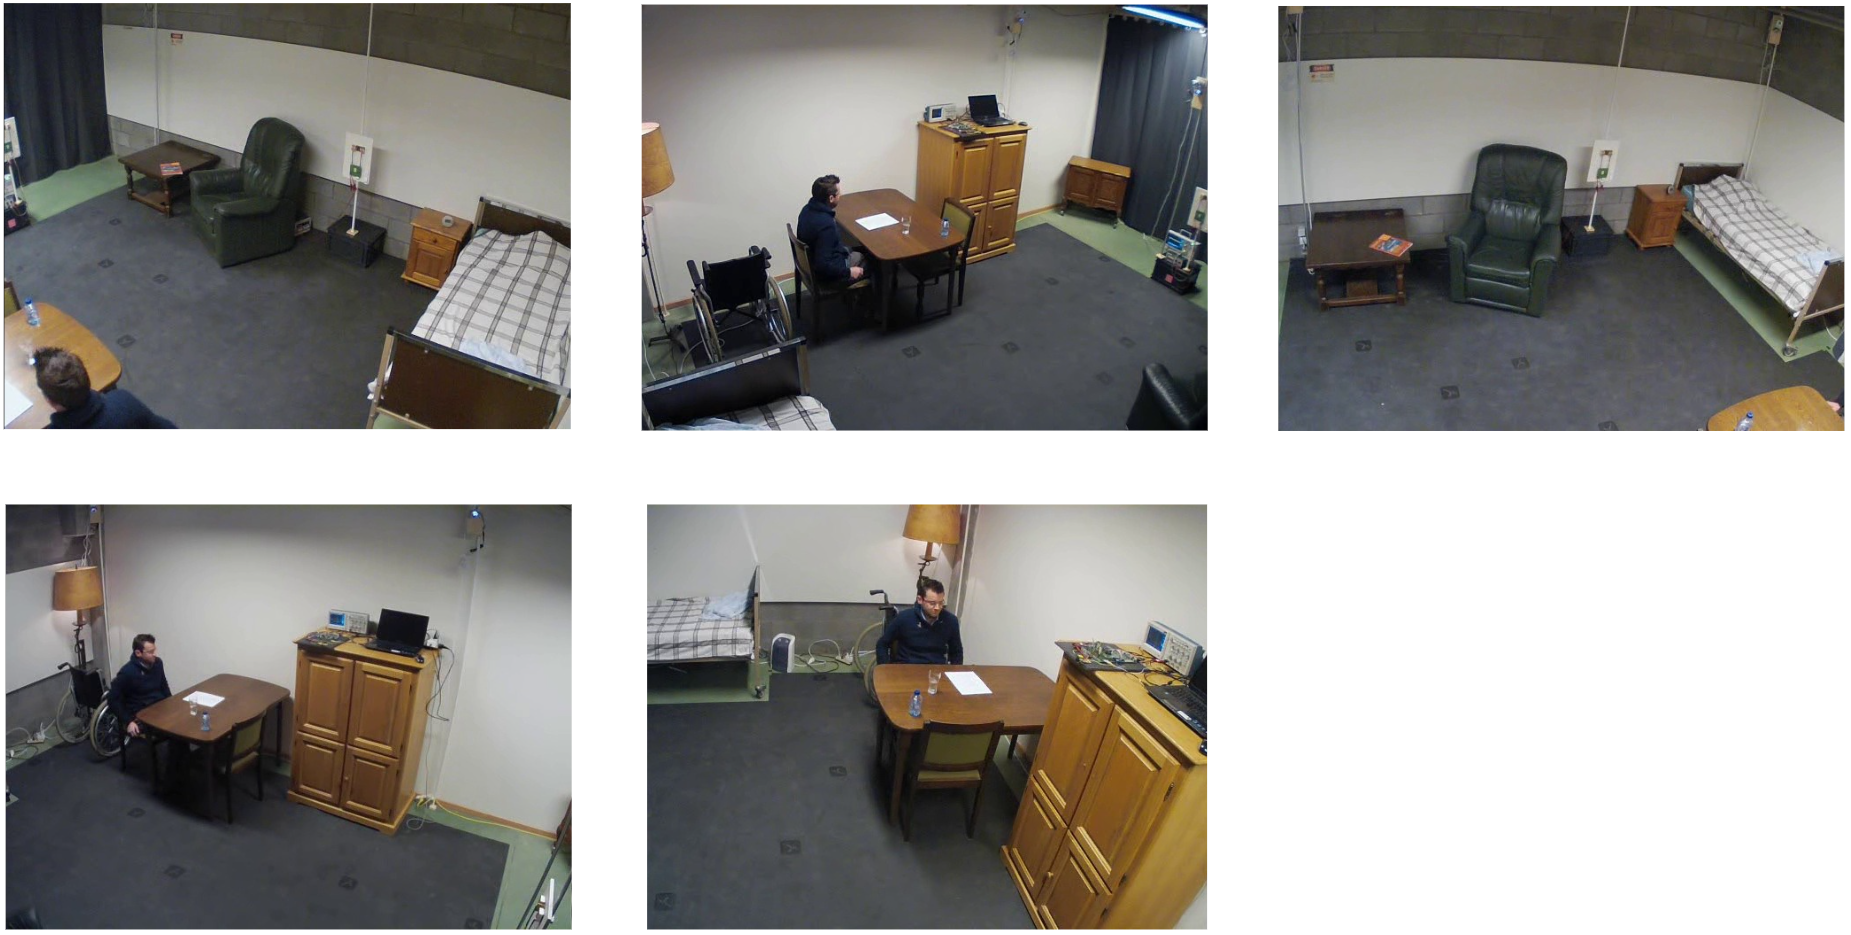
\includegraphics[width=0.6\textwidth]{figure/BAB 3/Preview 5 sudut kamera dataset.png}
    \caption{Preview of the dataset from five camera viewpoints.}
    \label{fig:preview 5 sudut kamera}
\end{figure}

The dataset consists of 54 fall scenarios and 17 non-fall scenarios. Each scenario was recorded from five different viewpoints, as shown in Figure \ref{fig:preview 5 sudut kamera}, resulting in 270 fall videos and 85 non-fall videos. The fall videos range from 1 to 5 minutes in duration, while the non-fall videos range from 10 to 30 minutes. All videos have a frame size of 800 $\times$ 480 pixels. A metadata file is also provided, containing detailed information for each video. For each fall video, the metadata include the actor, initial fall condition, final fall condition, and scenario description. In addition, the fall start time, the exact fall time, the end of the fall event, and the fall duration in seconds are provided. Similarly, for non-fall videos, the scenario description, video duration, and actor information are available. \par

\subsection{Data Preprocessing} \label{III.prapemrosesan}

\begin{figure}[H]
    \centering
    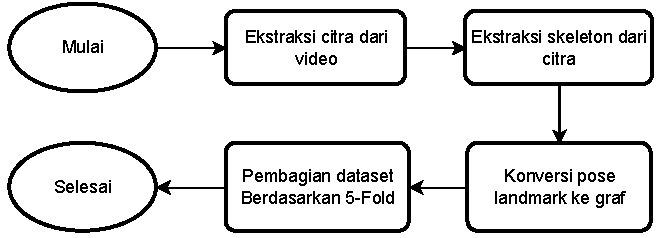
\includegraphics[width=0.55\textwidth]{figure/BAB 3/alur_prapemrosesan_dataset.pdf}
    \caption{Dataset preprocessing flow.}
    \label{fig: alur prapemrosesan}
\end{figure}

This subsection explains in detail the preprocessing flow required so that the dataset can be accepted by the model for training. As shown in Figure \ref{fig: alur prapemrosesan}, the preprocessing stage generally consists of four steps: extracting the required images from each video in the dataset, using Mediapipe Pose to detect 33 human pose landmarks from each image while also balancing the amount of data in each class when the class sizes are unequal, converting the pose landmark data into graph form, and finally splitting the data using 5-Fold to avoid data leakage during model training. All of these stages are necessary so that the GCN model can process and learn the spatial patterns and relationships among landmarks, enabling accurate prediction of fall and non-fall positions. \par

\subsubsection{Image Extraction from Video} \label{III.ekstrak citra}

The initial preprocessing step is performed by extracting 30 images from a time range in each video within the dataset. This step aims to reduce the amount of data to be processed and to ensure that the analysis is conducted only on relevant image frames, both for fall and non-fall events. To achieve this objective, a Python-based frame extraction program was developed to automatically extract images based on the timestamp information provided in the metadata file. \par

The metadata file contains timestamp information indicating the start and end of the event for fall videos. However, timestamps are not provided for non-fall videos; therefore, the start and end times of the event segments in non-fall videos must be determined manually. These data are then used to determine the appropriate time intervals for image extraction. \par

In general, the extraction program begins by opening and reading the dataset metadata file. The start and end timestamps of fall and non-fall events are then used as references to determine the beginning and end points of each event in every video. There are 270 fall videos and 85 non-fall videos. Based on the timestamps in the metadata, the program selects 30 frames that are randomly and evenly distributed across the duration of a fall event to obtain representative data from the event. For example, if the fall duration is 2 seconds, then 30 frames are selected within that duration. Meanwhile, because the number of fall and non-fall videos is unequal, the number of non-fall videos must be adjusted by dividing each video into several segments based on the actor’s activity so that the total number of non-fall video segments becomes 270. \par

The program then extracts the frames according to the specified timestamps using the OpenCV library, identifies the frame positions corresponding to the defined timestamps, and stores the extracted images in an appropriate format such as JPG. The following simple calculation illustrates the total number of image frames expected to be obtained. \par

\begin{align*}
    \text{Total images} &= (\text{total fall videos} \times 30) + (\text{total non-fall videos} \times 30) \label{eq:total citra}\\
    &= (270 \times 30) + (270 \times 30) = 8{,}100 + 8{,}100 = 16{,}200
\end{align*}
\vspace{7pt}

Based on this calculation, the estimated total number of extracted image frames is 16,200. The extracted frames are stored in a well-organized folder structure based on video identity and related information to facilitate further analysis. An example of image frames obtained from the dataset videos can be seen in Figure \ref{fig:contoh frame}. \par

\begin{figure}[H]
    \centering
    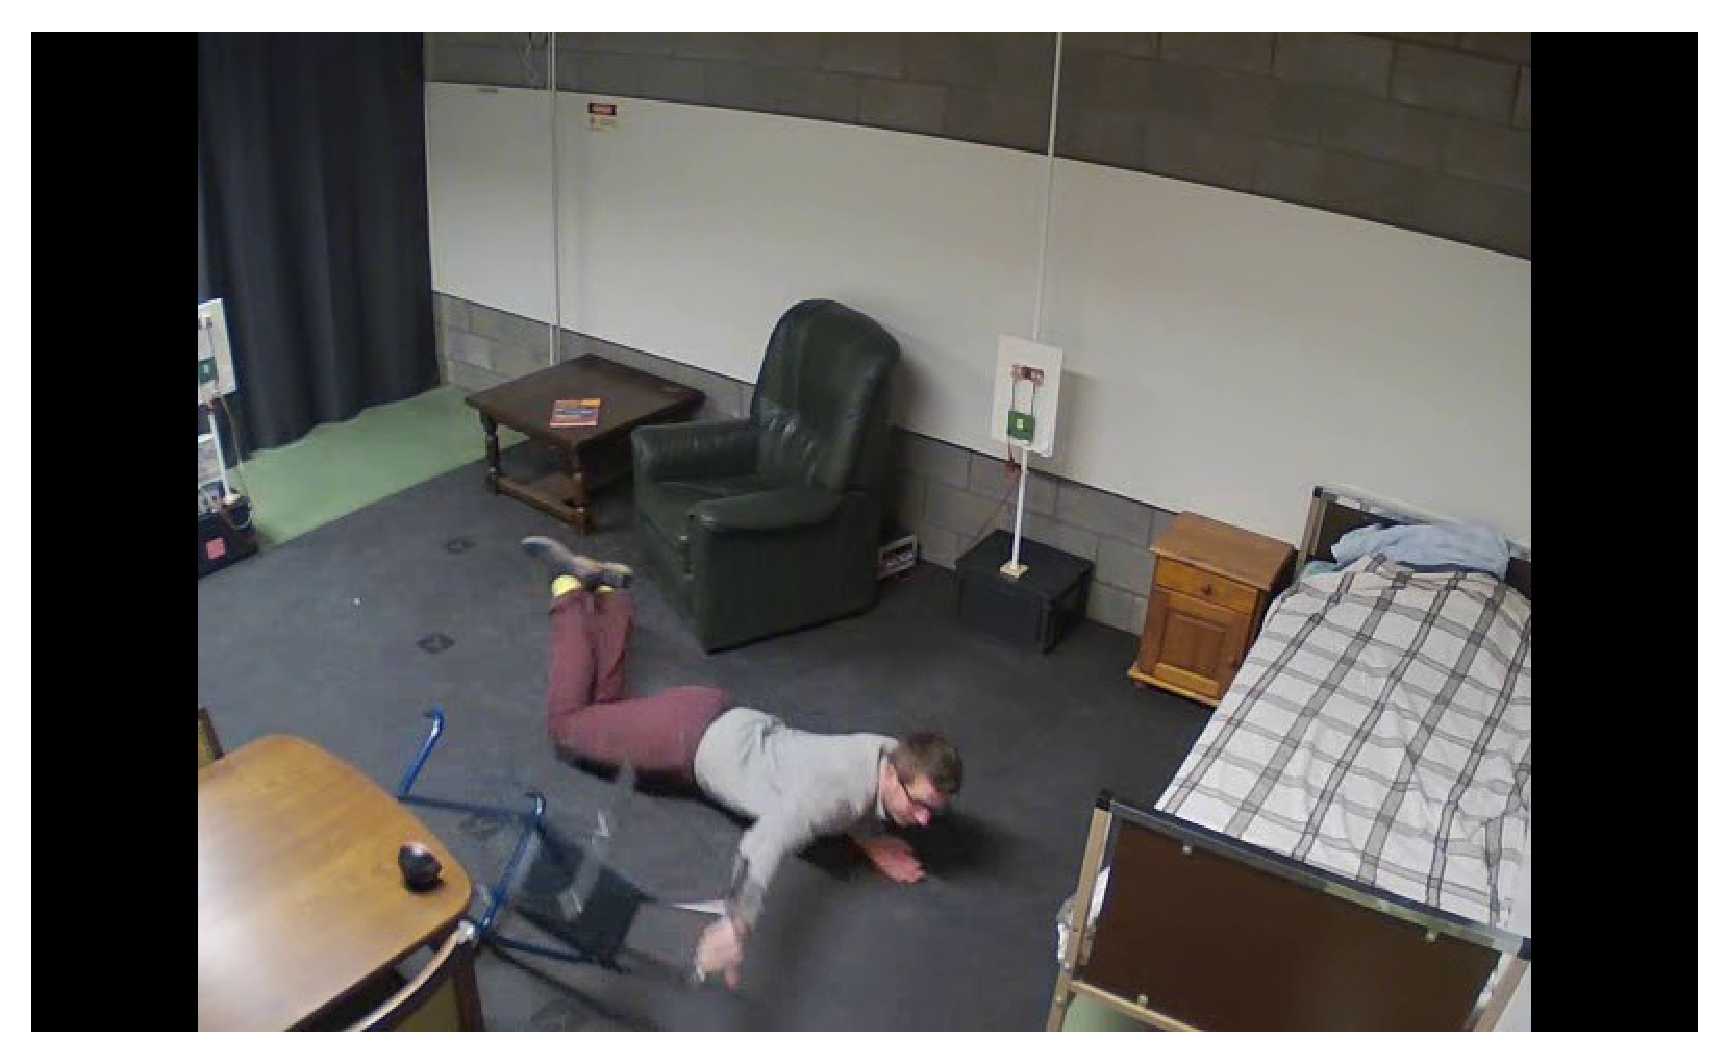
\includegraphics[width=0.4\textwidth, trim=3.5cm 0 3.5cm 0, clip]{figure/BAB 3/contoh citra jatuh.pdf}
    \caption{Example image frames from a fall video.}
    \label{fig:contoh frame}
\end{figure}

\subsubsection{Detection of 33 Landmarks Using Mediapipe Pose} \label{III.deteksi pose landmark}

The next process is that all extracted images are processed using the Mediapipe framework to obtain pose landmark data in JSON format. Before that, each image undergoes preprocessing through color conversion. If an image is originally in BGR format, it is converted into RGB format, since MediaPipe requires RGB input. Afterward, the image is processed to detect pose landmarks. The flow of the Mediapipe pose landmark detection process is shown in Figure \ref{fig:alur pose landmark}. \par

\begin{figure}[H]
    \centering
    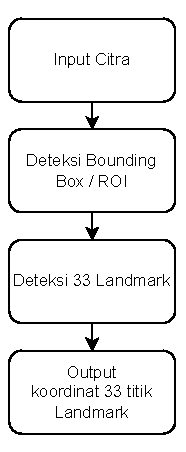
\includegraphics[width=0.15\textwidth]{figure/BAB 3/alur pemrosesan Pose Landmark.pdf}
    \caption{Flow of the pose landmark detection process.}
    \label{fig:alur pose landmark}
\end{figure}

There are two main processes performed in Mediapipe Pose using BlazePose. First, BlazePose detects the presence of the human body in the image and produces outputs in the form of a bounding box surrounding the body, as well as reference points such as the body center and body orientation. BlazePose determines the Region of Interest (ROI) that focuses on the human body area in the image. Second, BlazePose detects 33 coordinate points (landmarks) of the human body within the ROI. \par

\begin{figure}[H]
    \centering
    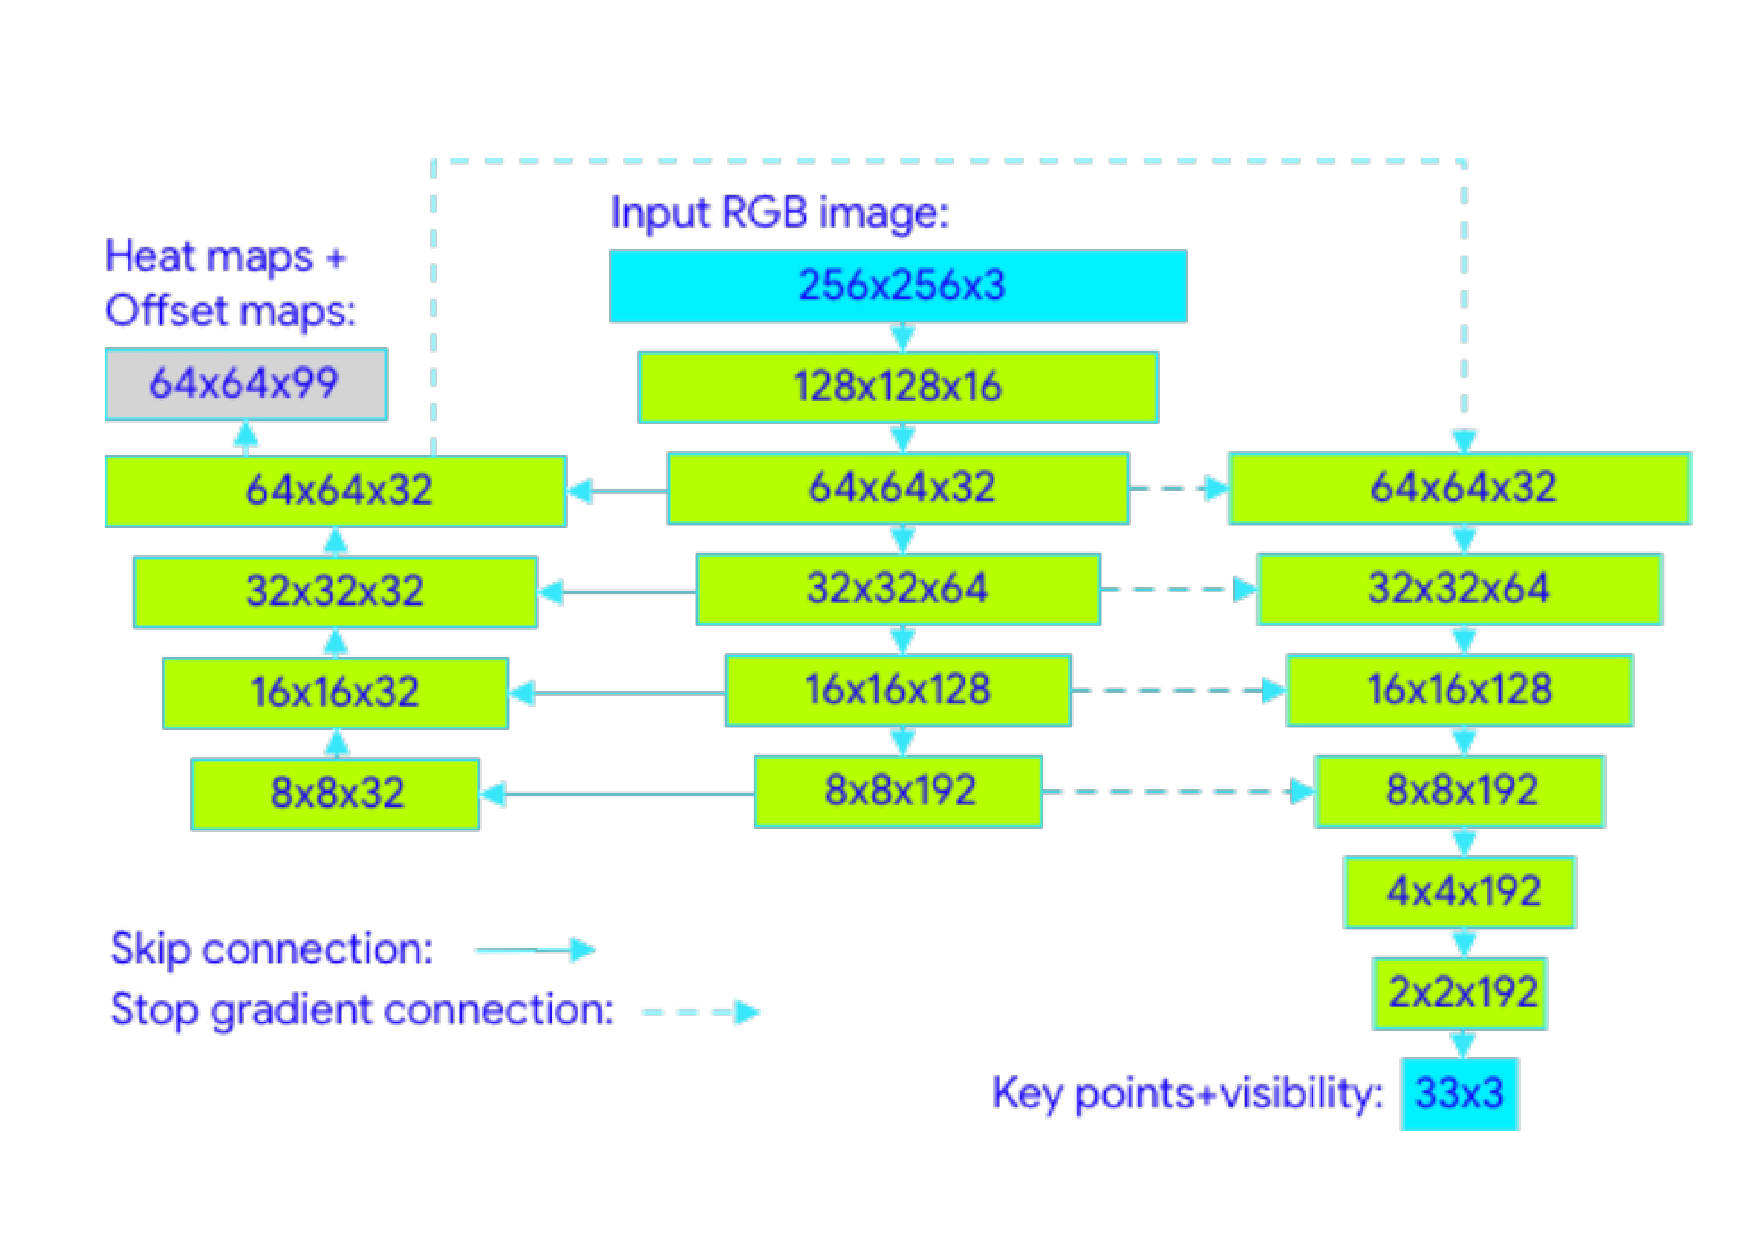
\includegraphics[width=0.55\textwidth]{figure/BAB 3/artisektur mediapipe pose.pdf}
    \caption{BlazePose network architecture \cite{bazarevsky2020}.}
    \label{fig:arsitektur mediapipe}
\end{figure}

The BlazePose network architecture uses a combination of heatmap, offset, and regression approaches to improve accuracy and efficiency in body pose detection, as shown in Figure \ref{fig:arsitektur mediapipe}. The process begins with an RGB image input of size 256$\times$256$\times$3, which has been processed automatically in the Mediapipe Pose framework. In the early stage of the pipeline, a person alignment proposal is generated to help the model focus on the relevant body area. Then, the heatmap layer is used only during the training phase of the BlazePose model to guide the learning process by providing a probability map indicating the possible position of each landmark, while the offset loss is used to correct the difference between predictions and the actual locations \cite{bazarevsky2020}. \par

At the inference stage, however, the output layers related to heatmap and offset are removed because the model has completed training. Therefore, only the regression network is used to estimate the landmarks with dimensions of 33$\times$3. This network utilizes skip-connections across all stages to combine high-level and low-level features, allowing the model to capture important information from various levels of complexity \cite{bazarevsky2020}. Based on this structure, BlazePose is able to detect human body pose landmarks with high accuracy, even on devices with limited computational resources. \par

\begin{figure}[H]
    \centering
    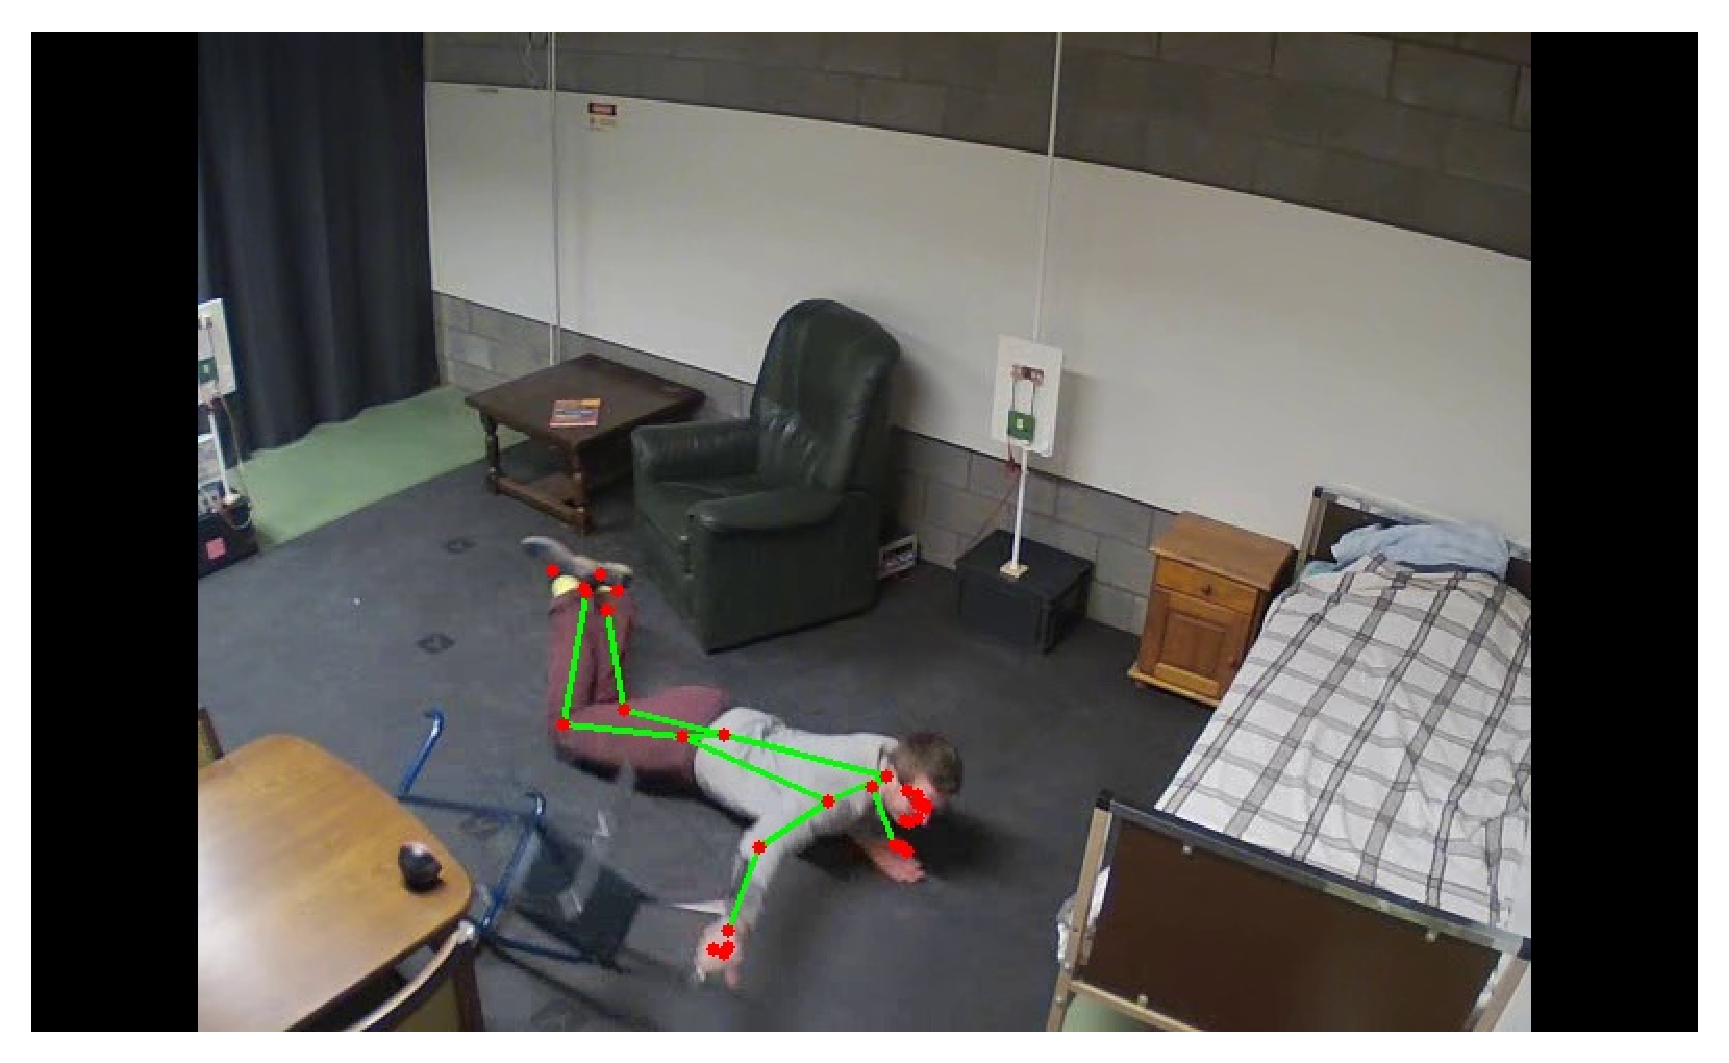
\includegraphics[width=0.4\textwidth, trim=3.5cm 0 3.5cm 0, clip]{figure/BAB 3/contoh deteksi landmark.pdf}
    \caption{Preview of landmark detection results on an image.}
    \label{fig:contoh preview landmark}
\end{figure}

An example of the preview of landmark detection results can be seen in Figure \ref{fig:contoh preview landmark}. Each landmark has x, y, and z attributes, where x and y describe the landmark position relative to the image coordinate system, while z describes the depth (3D) relative to the midpoint, with the reference point located around the hip area. The smaller the z value, the closer the landmark appears to the camera. All successfully detected landmarks in each image are stored separately in JSON files. An example of the stored data can be seen in Figure \ref{fig:contoh landmark json}. \par

\begin{figure}[H]
    \centering
    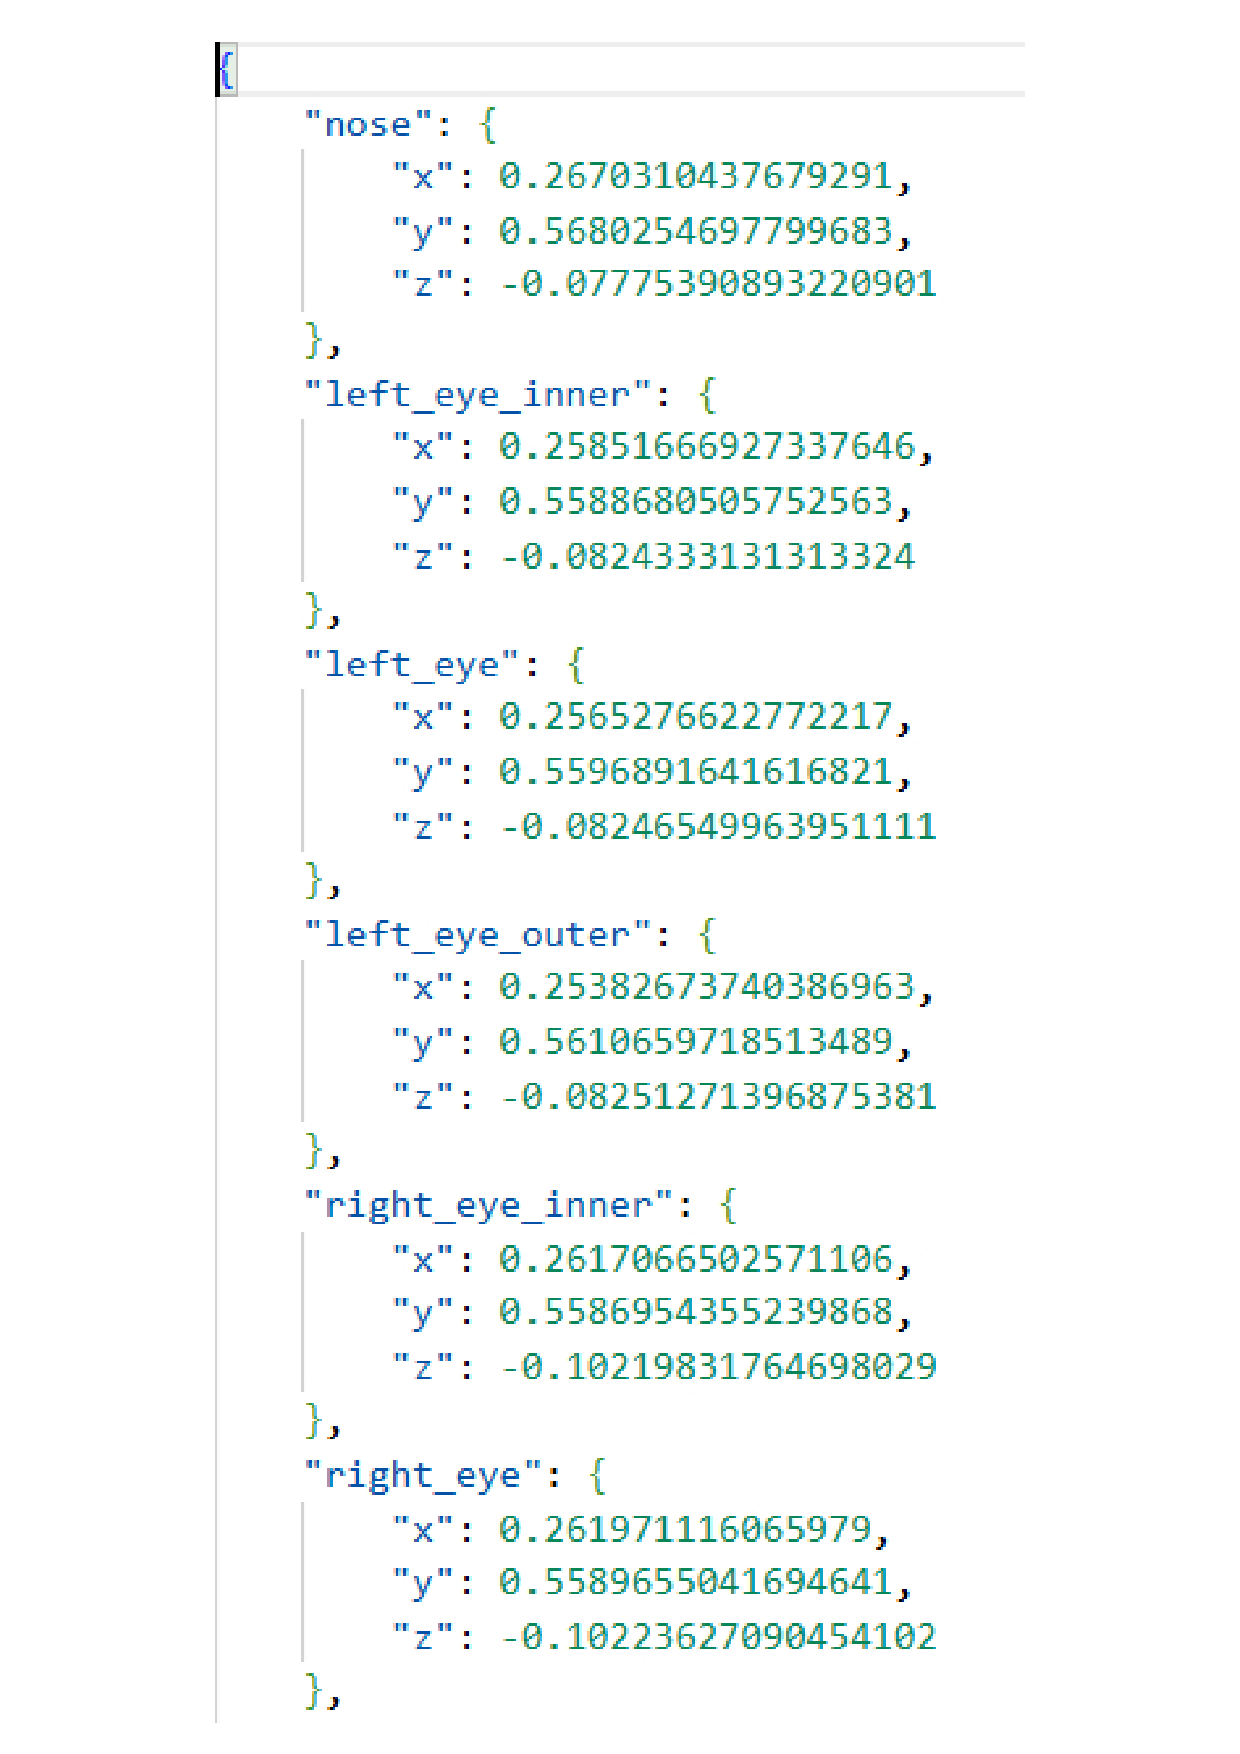
\includegraphics[width=0.4\textwidth]{figure/BAB 3/contoh data pose landmark.pdf}
    \caption{Example of pose landmark data.}
    \label{fig:contoh landmark json}
\end{figure}

\subsubsection{Conversion of Pose Landmark Data into Graphs} \label{III.konversi landmark ke graf}

After obtaining 33 landmarks from each image, the data must first be converted into graph format because the GCN model requires graph-structured data to process relationships among nodes. This conversion involves transforming the data into tensors containing node and edge information. The resulting graph data can then be used for training and prediction with the GCN model. The conversion flow is shown in Figure \ref{fig:alur konversi landmark graf}. \par

\begin{figure}[H]
    \centering
    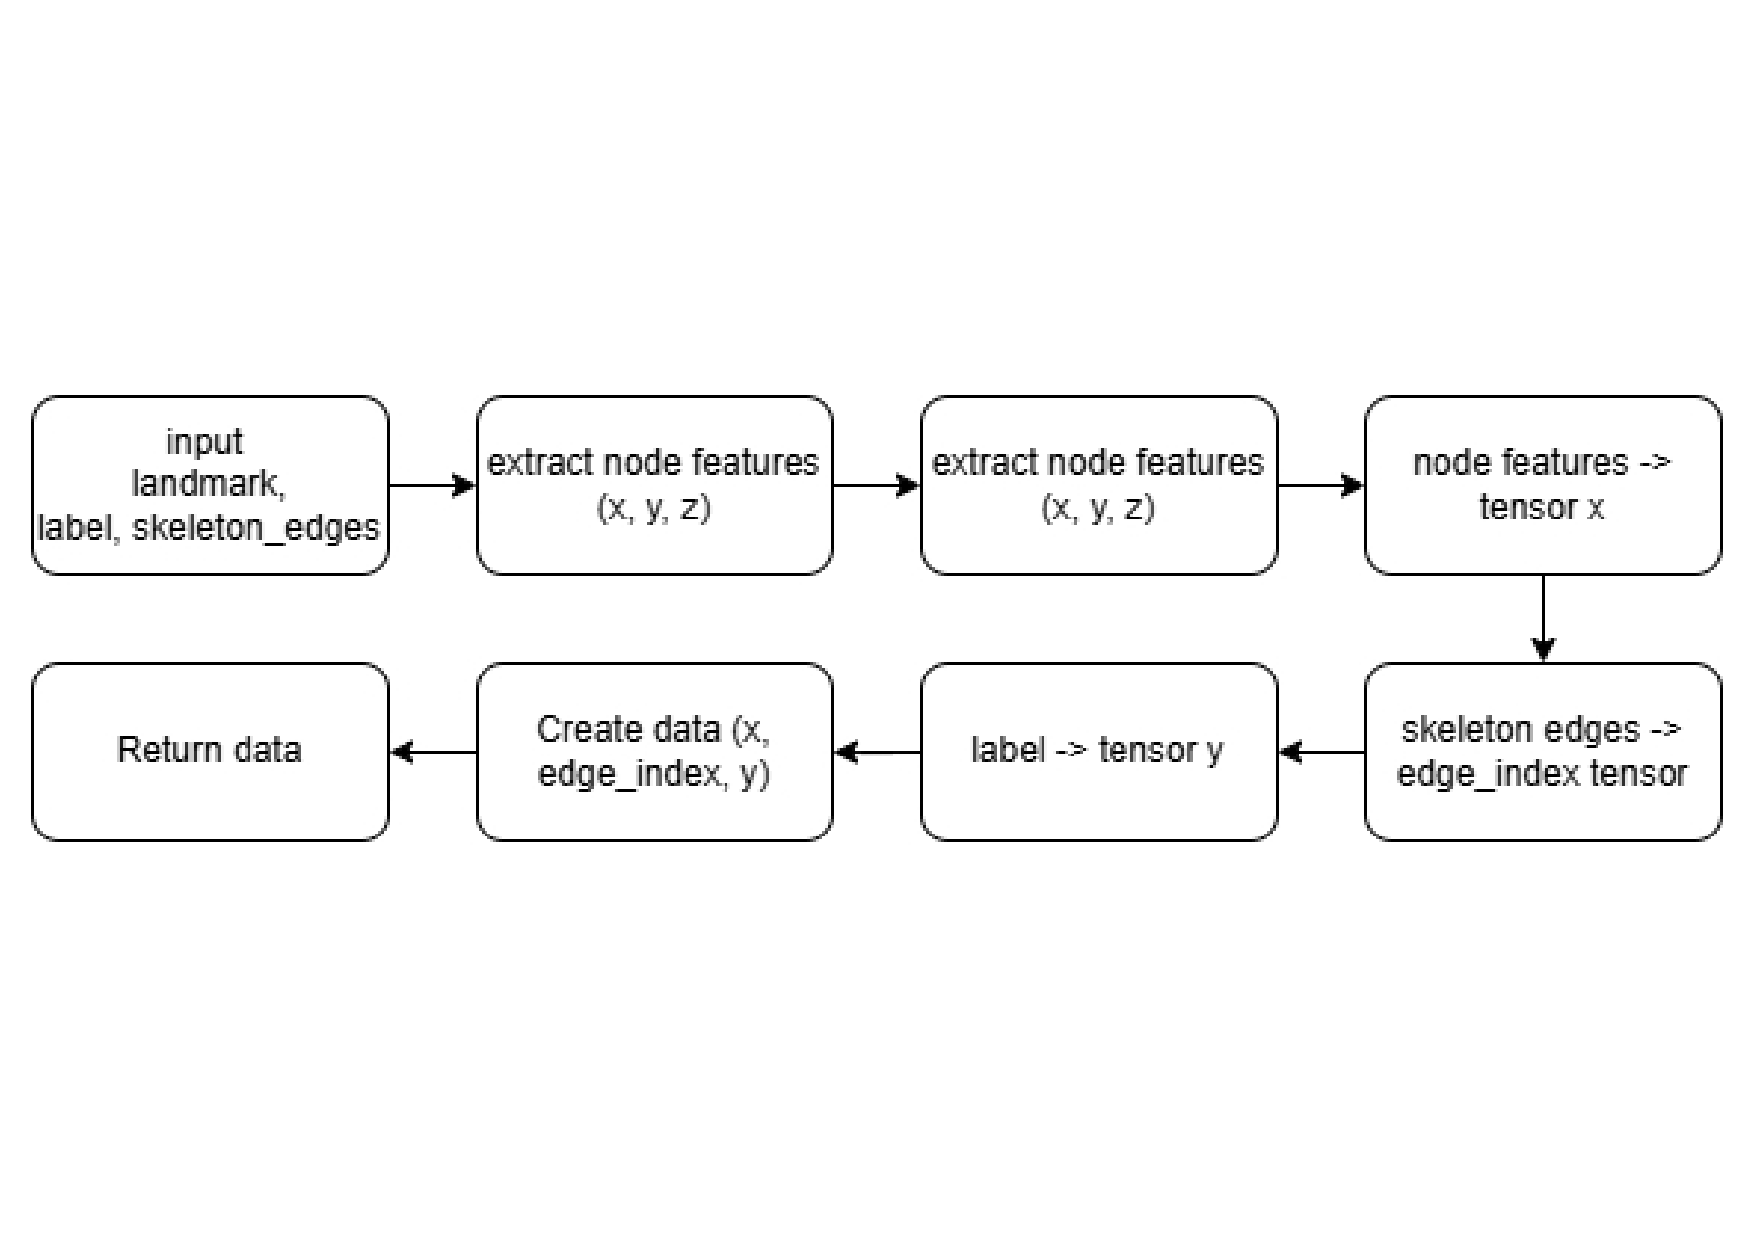
\includegraphics[width=0.4\textwidth]{figure/BAB 3/konversi pose landmark ke graf.pdf}
    \caption{Flow of converting pose landmark data into graph data.}
    \label{fig:alur konversi landmark graf}
\end{figure}

The conversion process begins with three inputs: landmark data, labels, and skeleton edges. Landmarks represent body points used to determine the pose, while skeleton edges describe the relationships or connections among the landmarks. The first step is to extract node features for each landmark, which consist of 3D coordinates (x, y, z). These features are then transformed into a tensor representing the positions of landmarks in three-dimensional space. After that, the skeleton edges, which describe the relations among landmarks, are transformed into a tensor containing the edge indices (relationships among nodes). The graph data are then constructed by combining the tensor of node features (x), the edge index tensor (edge\_index), and the label (y) to be predicted. The labels are also converted into tensors for further processing. Once all data have been converted into tensor format, they are returned as output ready to be used in graph modeling or further analysis. In this way, human pose data are transformed into graph representations ready to be processed by the model. \par

\subsubsection{K-Fold Data Splitting}

The next step is the application of the K-Fold dataset splitting technique. This technique divides the dataset into several parts called folds, allowing the creation of as many as $k$ subsets of fall and non-fall data to support model generalization while reducing the potential for overfitting. However, one consequence is that the training cycle requires more computational time and resources compared with conventional data-splitting schemes. Another important consideration is that if the value of $k$ is too large, the data in each fold become smaller, which may produce higher variance estimates, especially when the dataset is not sufficiently large. On the other hand, if the value of $k$ is too small, the risk of bias in the model error estimation may increase \cite{Hadjisolomou2021}. \par

The use of K-Fold with $K=5$ has been shown to be an effective choice in many applications and remains a good standard in many models. It provides a good balance between bias and variance and offers better computational efficiency than higher settings \cite{Hadjisolomou2021}. Therefore, this study adopts $k=5$. The first step in applying K-Fold is grouping the pose landmark dataset based on the folder prefix, which represents the recording session, so that data from the same subject are not mixed between the training and validation sets. The list of prefixes is then proportionally divided into five folds using the \texttt{KFold} function from scikit-learn. \par

\begin{figure}[H]
    \centering
    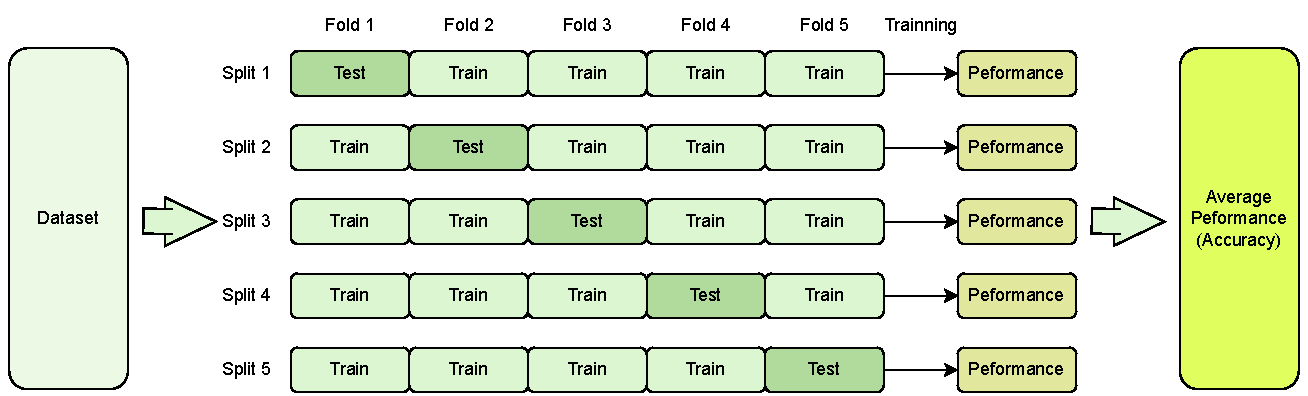
\includegraphics[width=0.9\textwidth]{figure/BAB 3/K-fold.pdf}
    \caption{Dataset splitting using 5-Fold.}
    \label{fig:k-fold}
\end{figure}

An illustration of dataset splitting using the K-Fold technique is shown in Figure \ref{fig:k-fold}. The entire fall and non-fall dataset is divided into five folds, with each fold containing 20\% of the total data. These five folds are then arranged into five split variations, each consisting of 80\% training data and 20\% evaluation data. In one full K-Fold cycle, the training process is performed five times using five different folds, where each fold trains a new model. This means that in this K-Fold training scheme, five models are trained using five different dataset split variations. \par

\subsection{GCN Model Design} \label{III.perancangan GCN}

This stage presents the design of the overall model-building pipeline. The design utilizes a Graph Convolutional Network (GCN) architecture inspired by ResGCN to effectively capture inter-node relationships through residual connections. Model tuning is performed by setting several key hyperparameters, including the optimizer type, learning rate, weight decay, batch size, dropout, number of epochs, hidden channel size, and residual activation to obtain optimal performance. \par

\begin{figure}[H]
    \centering
    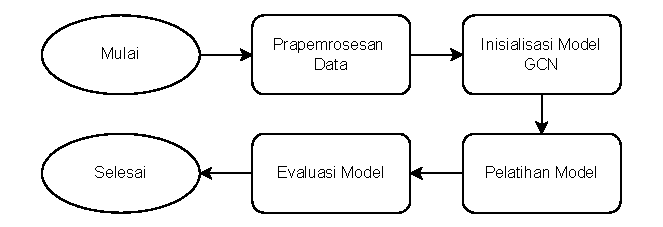
\includegraphics[width=0.6\textwidth]{figure/BAB 3/Diagram perancangan model gcn.pdf}
    \caption{Model design flow.}
    \label{fig:Alur perancangan model}
\end{figure}

Based on the design shown in Figure \ref{fig:Alur perancangan model}, the model design flow begins with the initial dataset consisting of labeled fall and non-fall videos, which must first be processed before being used for training. The preprocessing stage is carried out by extracting 30 images from each time segment in every video according to the guidelines in the meta file. Each image is then processed using MediaPipe Pose inference to obtain a body skeleton containing node coordinates and edge structures. All coordinates are stored as separate JSON files, with one JSON file for each image. The dataset is then split using a 5-Fold scheme to assess the quality of model training. Before being processed further, the coordinate data are converted into graph representations so that they can be accepted by the GCN model. \par

The GCN-based classification model is trained for the binary classification task of determining whether a graph represents a fall or a non-fall condition. The 5-fold scheme is used to divide the training and validation data while grouping images by video to prevent identity leakage across videos. During training, Binary Cross-Entropy (BCE) loss is used as the loss function. To assess consistency and learning efficiency, training is repeated five times with reinitialization, and each run is performed on a different fold. Evaluation focuses on accuracy and loss to assess the model’s ability to predict fall and non-fall positions in each image. \par

\begin{figure}[H]
    \centering
    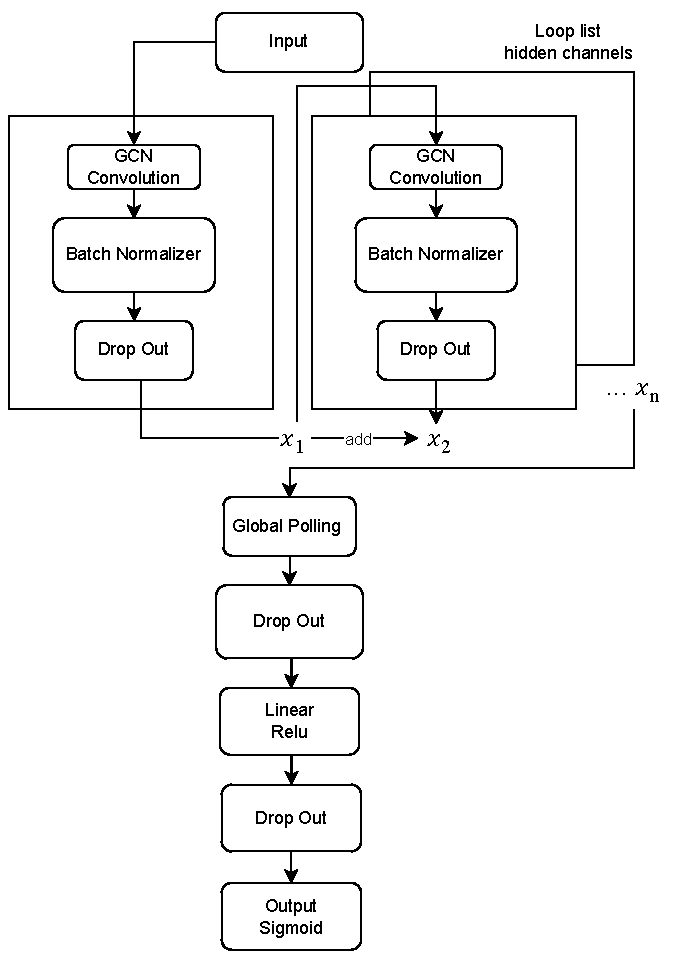
\includegraphics[width=0.55\textwidth]{figure/BAB 3/Arsitektur model GCN.pdf}
    \caption{Proposed GCN model architecture.}
    \label{fig:arsitektur model gcn}
\end{figure}

The GCN model is designed as shown in Figure \ref{fig:arsitektur model gcn}. The first layer receives input data in the form of pose landmark representations that have been converted into graphs. In the GCN convolution layer, the input data undergo a convolution process in which the GCN updates the features of each node based on the features of its neighboring nodes, enabling the model to exploit graph structure to produce better predictions. Next, a Batch Normalizer layer is used to normalize the output from the previous layer, helping reduce distribution shifts during training, accelerate the training process, and improve model stability. \par

A Dropout layer is used to prevent overfitting by randomly deactivating several units during training. This helps the model avoid depending too heavily on certain features and improves generalization. A Global Pooling layer is used to reduce data dimensionality after convolution by aggregating information from the entire graph and summarizing important features into a more compact representation. Next, a Linear layer with ReLU activation is added to transform the processed information into a representation suitable for classification or prediction. The final fully connected layer with sigmoid activation converts the model output into probabilities used for two-class classification, namely fall and non-fall. \par

This architecture is selected because it can prevent performance degradation that often appears in graph networks through the implementation of residual learning, namely skip-connections, which preserve gradient flow and prevent oversmoothing of node features. This architecture extracts node representations through GCNConv layers, stabilizes them with Batch Normalization, and then summarizes all nodes into a single graph vector using global pooling. The residual skip-connection is employed to mitigate oversmoothing when the number of layers increases, before the final representation is processed by the MLP head to generate prediction probabilities. \par

\subsection{Model Training} \label{III.pelatihan}

After the model architecture has been constructed, the next step is model training. At this stage, the GCN model is trained using the dataset that has already been processed and split using the 5-Fold technique as described in Subsection \ref{III.prapemrosesan}. The training process involves learning body-position patterns and other activities of older adults based on the pose landmark data. The model is trained using several hyperparameters with default values, as shown in Table \ref{table:3. hyperparamter default}, and also through an ablation study whose details are presented in the relevant table. \par

\subsection{Model Evaluation} \label{III.evaluasi}

After the model has been trained, the next step is performance evaluation. At this stage, the model is tested using data that are not involved in training, namely the 20\% test portion provided in each fold, to measure accuracy, precision, recall, and F1-Score. The evaluation focuses primarily on the accuracy metric to determine how precisely the model is able to detect fall positions in older adults. To obtain the overall performance value, the five accuracy values obtained from each fold are averaged. \par

\subsubsection{Main Experiment Using Default Hyperparameter Settings} \label{III.evaluasi default}

This subsection presents the hyperparameter values used in the main experiment to test the model’s ability to classify fall and non-fall positions across the entire dataset. The training is conducted using default hyperparameter settings formulated from common practice in the literature and the PyTorch documentation. The values used for Optimizer, Learning Rate, Weight Decay, Batch Size, DropOut, Epoch, Hidden Channel, and Residual are summarized in Table \ref{table:3. hyperparamter default} as the reference configuration for the main experiment before further exploration.

\begin{table}[ht]
    \centering
    \caption{Default Values of Model Hyperparameters.}
    \label{table:3. hyperparamter default}
    \begin{tabular}{ c c c }
        \hline
        \textbf{No} & \textbf{Hyperparameter} & \textbf{Default Value} \\
        \hline
        1 & Optimizer & AdamW \\
        2 & Learning Rate & 1e-3 \\
        3 & Weight Decay & 1e-5 \\
        4 & Batch Size & 32 \\
        5 & DropOut & 0.3 \\
        6 & Epoch & 100 \\
        7 & Hidden Channel & [64, 32, 32, 32, 32] \\
        8 & Residual & True \\
        \hline
    \end{tabular}
\end{table}

Tabel \ref{table:3. hyperparamter default} summarizes the basic configuration used in the main experiment as a consistent starting point for GCN-based fall/non-fall classification. AdamW is selected as the optimizer because it is stable for small- to medium-scale graph learning and tends to provide good generalization. A learning rate of 1e-3 is used as an initial value that is sufficiently aggressive while still remaining stable, whereas a weight decay of 1e-5 is set to provide mild regularization and suppress overfitting on skeleton pose data. A batch size of 32 balances gradient estimation stability and memory limitations, while a dropout value of 0.3 is applied to the representation layers to control model complexity. The training process is run for 100 epochs while still applying early stopping to allow convergence without overtraining, with a hidden channel configuration of [64, 32, 32, 32, 32] as a compromise between representational capacity and computational efficiency. In addition, residual connection is enabled (True) to facilitate gradient flow across stacked GCN layers and improve training stability. This configuration serves as the baseline reference for the basic experiment before further exploration in Subsection \ref{III.evaluasi ablasi}. \par

\subsubsection{Additional Experiment Based on Ablation Study} \label{III.evaluasi ablasi}

This subsection presents additional experiments in the form of an ablation study to evaluate the contribution and sensitivity of key components in the GCN model. An ablation study is an experimental procedure in which one factor is varied at a time while the remaining factors are kept at the default configuration to isolate the influence of that factor on model performance. Its main objective is to identify the most influential components, understand the trade-off in performance, and obtain a configuration that is more robust to data variation. This approach helps determine whether performance improvements arise from a particular adjustment, such as the optimizer or learning rate, or merely from uncontrolled combinations of settings. \par

The ablation study in this subsection focuses on five core hyperparameters that are considered most likely to influence learning dynamics, namely Optimizer, Learning Rate, Weight Decay, Batch Size, and DropOut. Each variation is tested while keeping the remaining components at the default configuration defined in the main experiment, and the results are evaluated using accuracy, recall, precision, and F1-score so that the outcomes can be compared fairly. The range of values and variation scenarios for each hyperparameter are summarized in Table \ref{table:3. ablasi hyperparamter} as the reference for conducting and interpreting the ablation study. \par

\begin{table}[ht]
    \centering
    \caption{Variations of Model Hyperparameters.}
    \label{table:3. ablasi hyperparamter}
    \begin{tabular}{c c c}
        \hline
        \textbf{No} & \textbf{Hyperparameter} & \textbf{Variation} \\
        \hline
        1 & Optimizer & \parbox[t]{5cm}{\centering 1. AdamW \\ 2. RMSProp \\ 3. LION} \\ \\
        2 & Learning Rate & \parbox[t]{4cm}{\centering 1. 0.01 or 1e-2 \\ 2. 0.001 or 1e-3 \\ 3. 0.0001 or 1e-4} \\ \\
        3 & Weight Decay & \parbox[t]{4cm}{\centering 1. 1e-4 \\ 2. 1e-5 \\ 3. 1e-6} \\ \\
        4 & Batch Size & \parbox[t]{4cm}{\centering 1. 16 \\ 2. 32 \\ 3. 64} \\ \\
        5 & DropOut & \parbox[t]{4cm}{\centering 1. 0.2 \\ 2. 0.3 \\ 3. 0.4} \\ \\
        - & Epoch & 100 \\
        - & Hidden Channel & [64, 32, 32, 32, 32] \\
        - & Residual & True \\
        \hline
    \end{tabular}
\end{table}

Table \ref{table:3. ablasi hyperparamter} summarizes the variation space used in this ablation study, where each experiment modifies only one hyperparameter while the others are locked to the default configuration. The Optimizer variation compares AdamW, RMSProp, and LION to assess differences in gradient dynamics, convergence stability, and implicit regularization in pose graphs. The learning rate is varied at the scale of \{1e-2, 1e-3, 1e-4\} to observe sensitivity in learning speed, accuracy, and training stability. Weight decay is tested at three values, namely \{1e-4, 1e-5, 1e-6\}, to examine the influence of regularization on generalization. Batch size values of \{16, 32, 64\} are selected to evaluate the trade-off among gradient noise, memory usage, and throughput, while DropOut values of \{0.2, 0.3, 0.4\} are analyzed as controls for graph representation complexity. Meanwhile, epoch 100, hidden channel [64, 32, 32, 32, 32], and residual True are not varied and are kept fixed to limit the search space so that comparisons remain focused. All variations are evaluated using accuracy and loss in a 1-fold scheme, where the selected fold is the one that achieved the best training accuracy in the main experiment. The results of this ablation study are expected to provide the basis for identifying the most influential configuration and the best candidate setting. \par


\section{RESULT AND ANALYSIS}
\label{}

This section presents the experimental results of the proposed Graph Convolutional Network (GCN) for elderly fall-position classification based on pose landmarks. The discussion covers dataset characteristics, preprocessing, model design, default training results, primary data testing, ablation study, and comparison between the default and optimized settings.

\subsection{Dataset Characteristics}
\label{IV.analisis}

The dataset consists of videos representing fall and non-fall activities in a realistic 2D camera setting. Example frames from both classes are shown in Fig. \ref{fig:data jatuh} and Fig. \ref{fig:data tidak jatuh}. For fall videos, the distribution is described based on the actor's initial position before the fall event. For non-fall videos, the distribution represents the actor's posture throughout the video. Three fall videos were missing from the original dataset, resulting in 267 fall videos and 270 non-fall videos.

\begin{figure}[H]
    \centering
    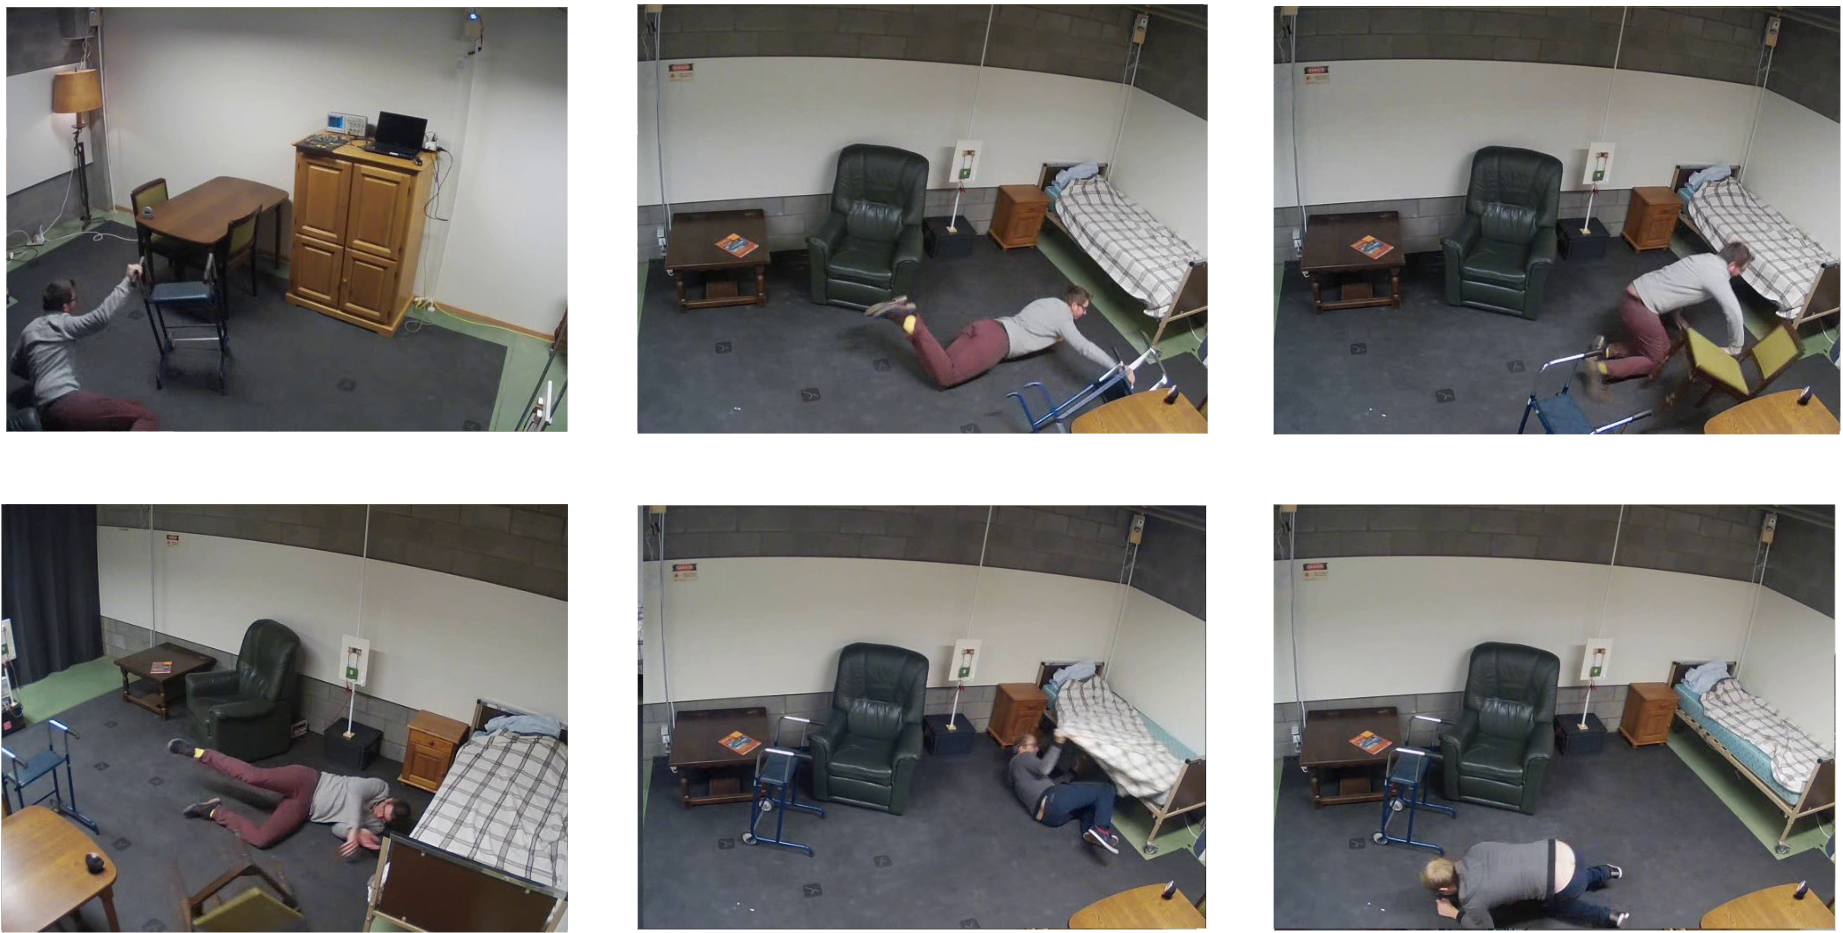
\includegraphics[width=0.55\textwidth]{figure/BAB 4/contoh fall.png}
    \caption{Examples of fall dataset videos}
    \label{fig:data jatuh}
\end{figure}

\begin{figure}[H]
    \centering
    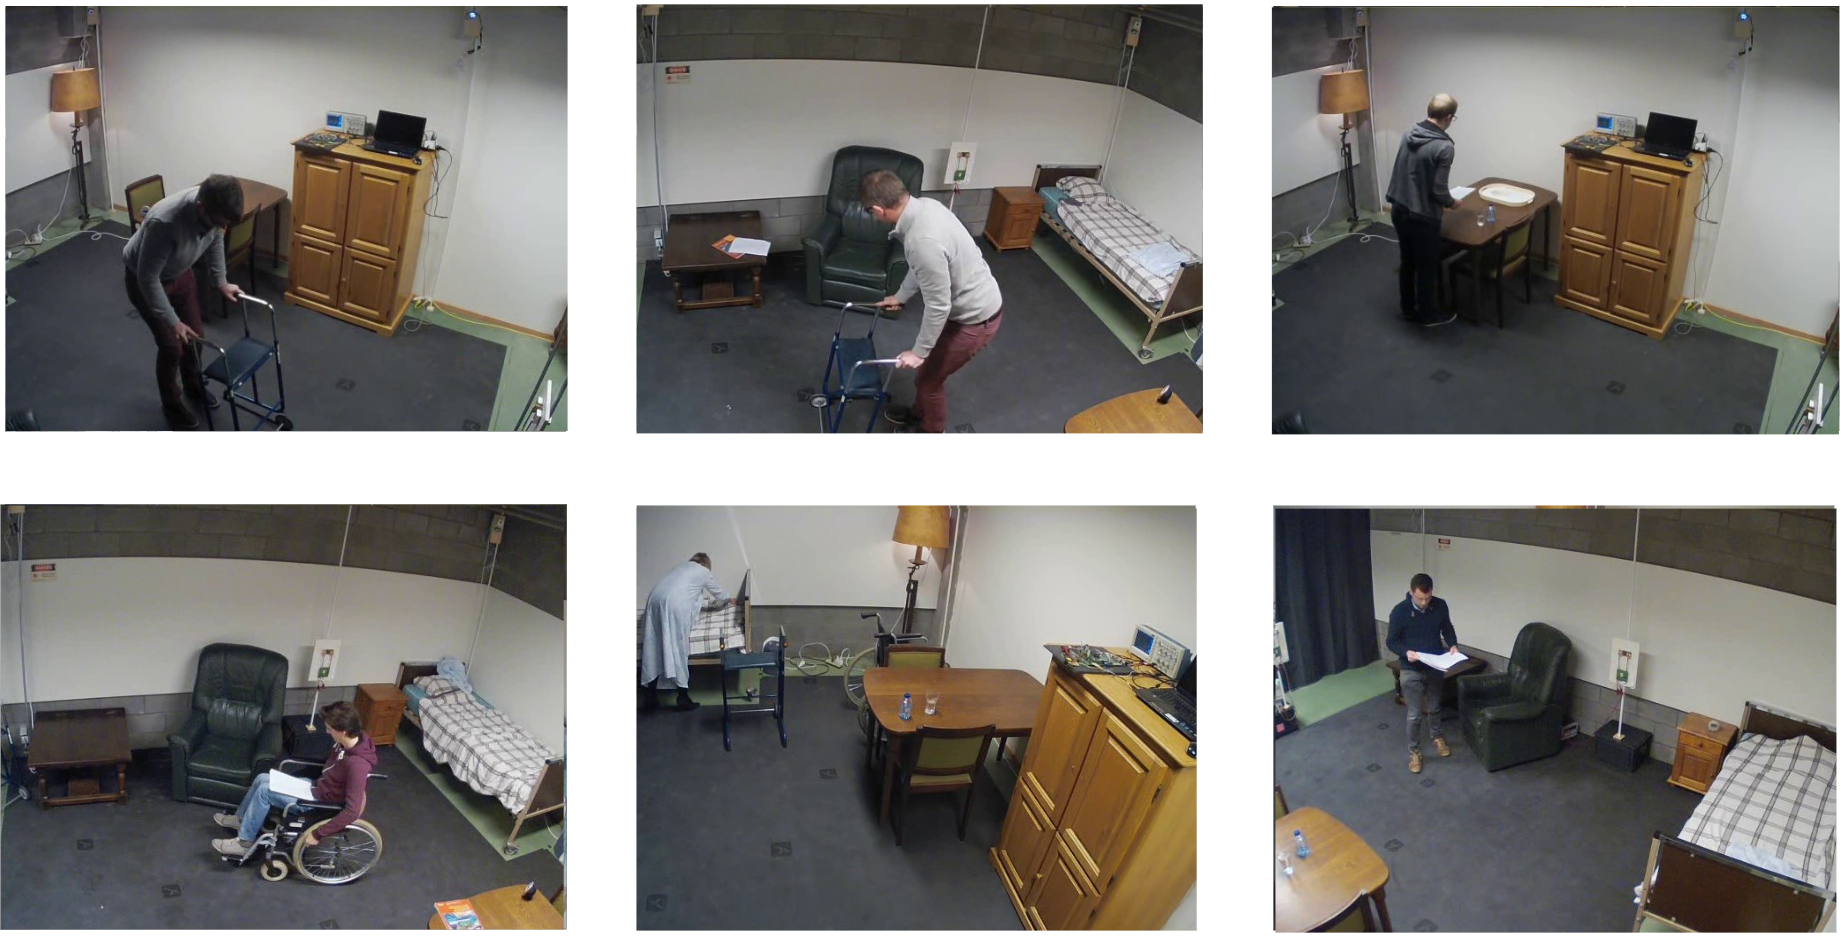
\includegraphics[width=0.55\textwidth]{figure/BAB 4/contoh not fall.png}
    \caption{Examples of non-fall dataset videos}
    \label{fig:data tidak jatuh}
\end{figure}

\begin{table}[H]
    \centering
    \caption{Distribution of fall videos}
    \label{table:4.data jatuh}
    \begin{tabular}{c c c}
        \hline
        \textbf{No} & \textbf{Initial Position} & \textbf{Total} \\ \hline
        1 & Standing & 117 \\ 
        2 & Standing-to-sitting transition & 35 \\ 
        3 & Sitting-to-standing transition & 10 \\ 
        4 & Kneeling & 30 \\ 
        5 & Bending & 25 \\ 
        6 & Sitting & 50 \\ \hline
        \multicolumn{2}{c}{\textbf{Total}} & \textbf{267} \\ \hline
    \end{tabular}
\end{table}

\begin{table}[H]
    \centering
    \caption{Distribution of non-fall videos}
    \label{table:4.data tidak jatuh}
    \begin{tabular}{c c c}
        \hline
        \textbf{No} & \textbf{Posture Throughout the Video (Start--End)} & \textbf{Total} \\ \hline
        1 & Standing & 65 \\ 
        2 & Standing-to-sitting transition & 80 \\ 
        3 & Sitting-to-standing transition & 35 \\ 
        4 & Bending & 75 \\ 
        5 & Sitting & 15 \\ \hline
        \multicolumn{2}{c}{\textbf{Total}} & \textbf{270} \\ \hline
    \end{tabular}
\end{table}

\subsection{Dataset Preprocessing}
\label{IV.prapemrosesan}

The preprocessing stage includes frame extraction, pose landmark detection, graph conversion, class balancing, and 5-fold splitting. This stage is essential because it determines the quality and consistency of the input used by the GCN model.

\subsubsection{Frame Extraction}
\label{IV.ekstrak frame}

Video metadata were read from an Excel file containing video paths, start and end times, and labels. Each video contributed 30 randomly extracted frames. In total, 537 folders and 16,110 frames were generated for the next stage.

\begin{table}[H]
    \centering
    \caption{Total frame extraction from videos}
    \label{tab:total citra}
    \begin{tabular}{c c c c c}
        \hline
        \textbf{No} & \textbf{Video Type} & \textbf{Total Videos} & \textbf{Frames per Video} & \textbf{Total Frames} \\ \hline
        1 & Fall & 267 & 30 & 8,010 \\ 
        2 & Non-fall & 270 & 30 & 8,100 \\ \hline
        \multicolumn{4}{c}{\textbf{Total Frames}} & \textbf{16,110} \\ \hline
    \end{tabular}
\end{table}

Table \ref{tab:total citra} shows that 8,010 frames were extracted from fall videos and 8,100 frames from non-fall videos. These frames were then used for detecting 33 body pose landmarks with MediaPipe Pose.

\subsubsection{Detection of 33 Pose Landmarks Using MediaPipe Pose}
\label{IV.ekstrak skeleton}

The output of pose.process returns results.pose\_landmarks, which contains 33 anatomical points in normalized coordinates within the range [0,1]. This normalization makes the representation independent of the original image resolution and simplifies later graph construction. A preview is shown in Fig. \ref{fig:preview pose landmark}.

\begin{figure}[H]
    \centering
    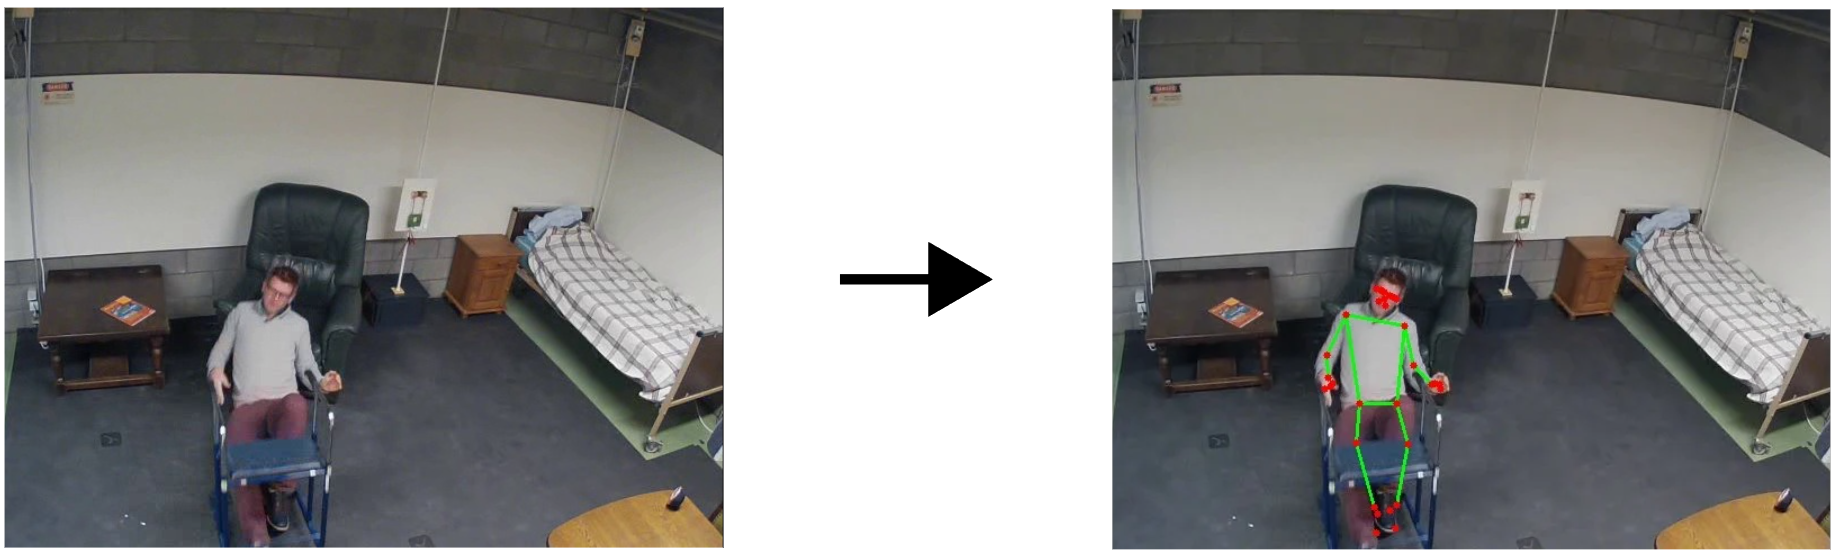
\includegraphics[width=0.6\textwidth]{figure/BAB 4/preview konversi citra ke pose lanmark.png}
    \caption{Preview of image to pose landmark conversion}
    \label{fig:preview pose landmark}
\end{figure}

A total of 6,292 frames failed during pose extraction because the confidence score was below 0.5. This failure affected 41 folders. As a result, 4,750 fall skeletons and 5,068 non-fall skeletons were successfully generated. To avoid class imbalance, non-fall skeletons were randomly reduced to match the fall class, producing 9,500 balanced skeleton samples in total.

\begin{table}[H]
    \centering
    \caption{Total skeleton extraction from frames}
    \label{tab:total skeleton}
    \begin{tabular}{c c c c c c}
        \hline
        \multirow{2}{*}{\textbf{No}} & \multirow{2}{*}{\textbf{Image Type}} & \multirow{2}{*}{\textbf{Total Frames}} & \multicolumn{3}{c}{\textbf{Skeleton Extraction}} \\ \cline{4-6}
        & & & \textbf{Successful} & \textbf{Failed} & \textbf{Balanced Total} \\ \hline
        1 & Fall & 8,010 & 4,750 & 3,260 & 4,750 \\
        2 & Non-fall & 8,100 & 5,068 & 3,032 & 4,750 \\ \hline
        \multicolumn{5}{c}{\textbf{Total}} & \textbf{9,500} \\ \hline
    \end{tabular}
\end{table}

Figure \ref{fig:contoh citra gagal diproses mediapipe} shows examples of frames that could not be processed by MediaPipe Pose, mainly because part of the body was cropped, which reduced the confidence score below the threshold.

\begin{figure}[H]
    \centering
    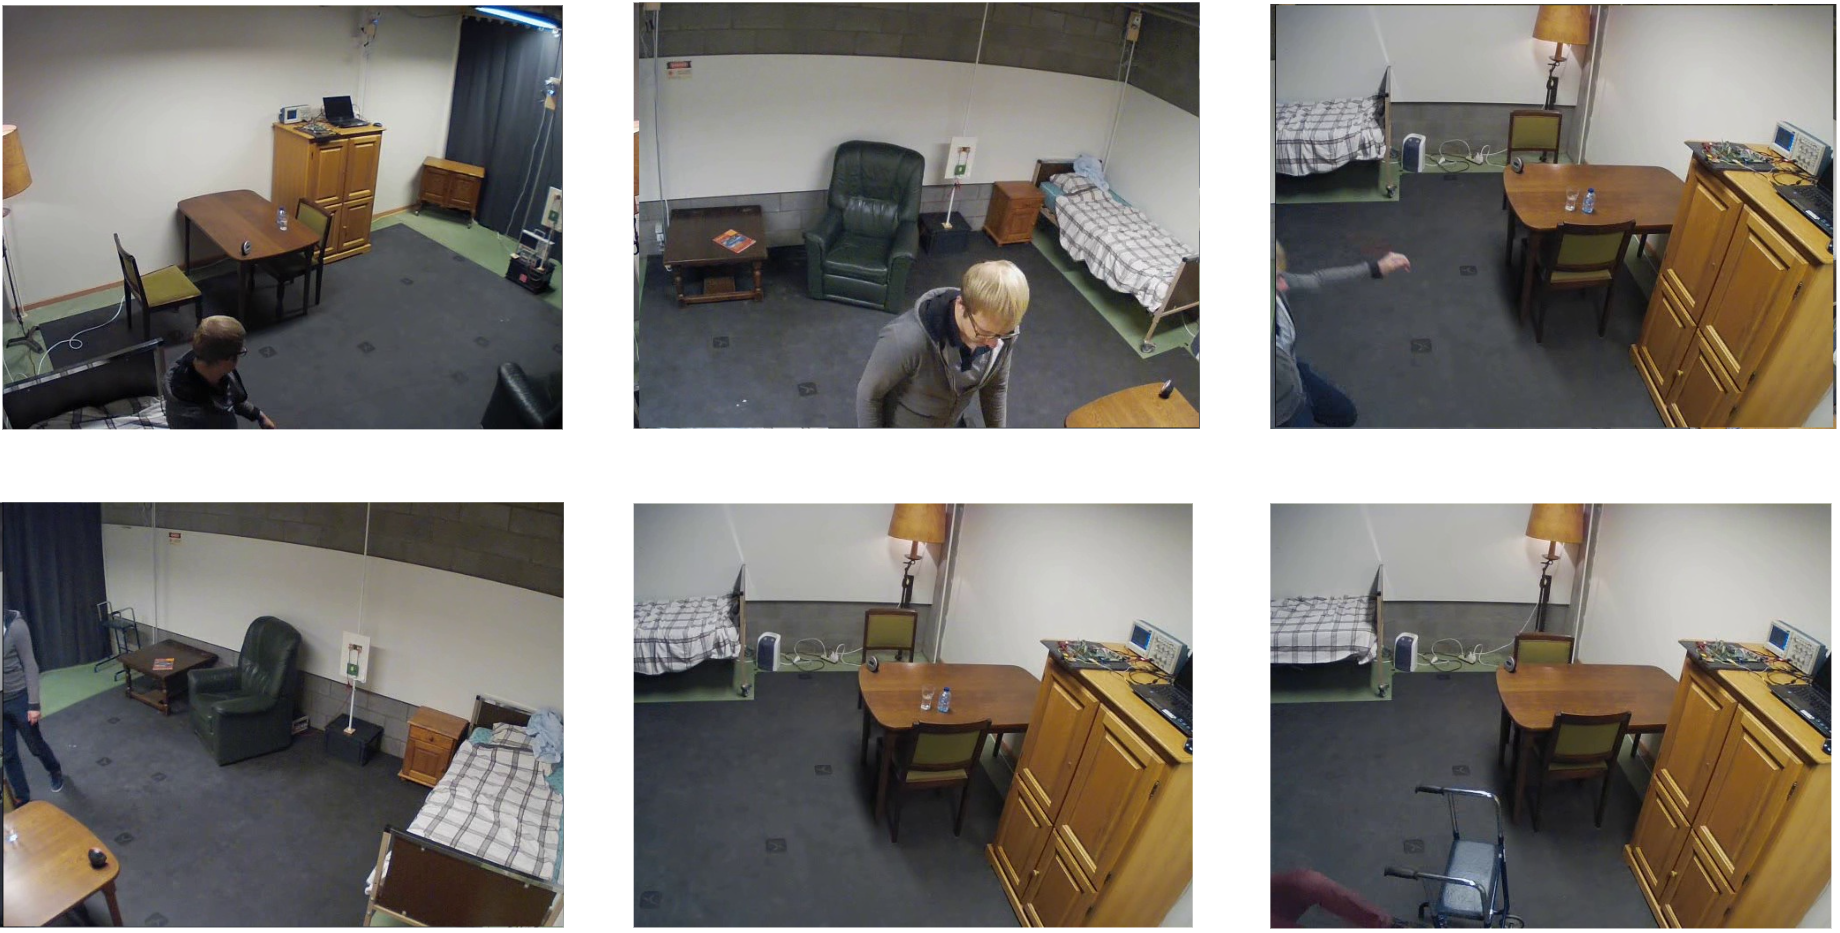
\includegraphics[width=0.6\textwidth]{figure/BAB 4/contoh citra gagal diproses mediapipe.png}
    \caption{Examples of frames that failed to be processed by MediaPipe Pose}
    \label{fig:contoh citra gagal diproses mediapipe}
\end{figure}

\subsubsection{Conversion of Pose Landmarks into Graphs}
\label{IV.konversi graf}

Each skeleton sample was converted into graph data using Kode \ref{kode:skeleton edges} and Kode \ref{kode:konversi skeleton graf}. The graph contains node features, edge indices, and class labels. Each node stores three features that represent coordinate information, while the graph contains 29 edges to model body-joint relations. This representation allows the model to learn spatial dependencies between body landmarks.

\begin{figure}[H]
    \centering
    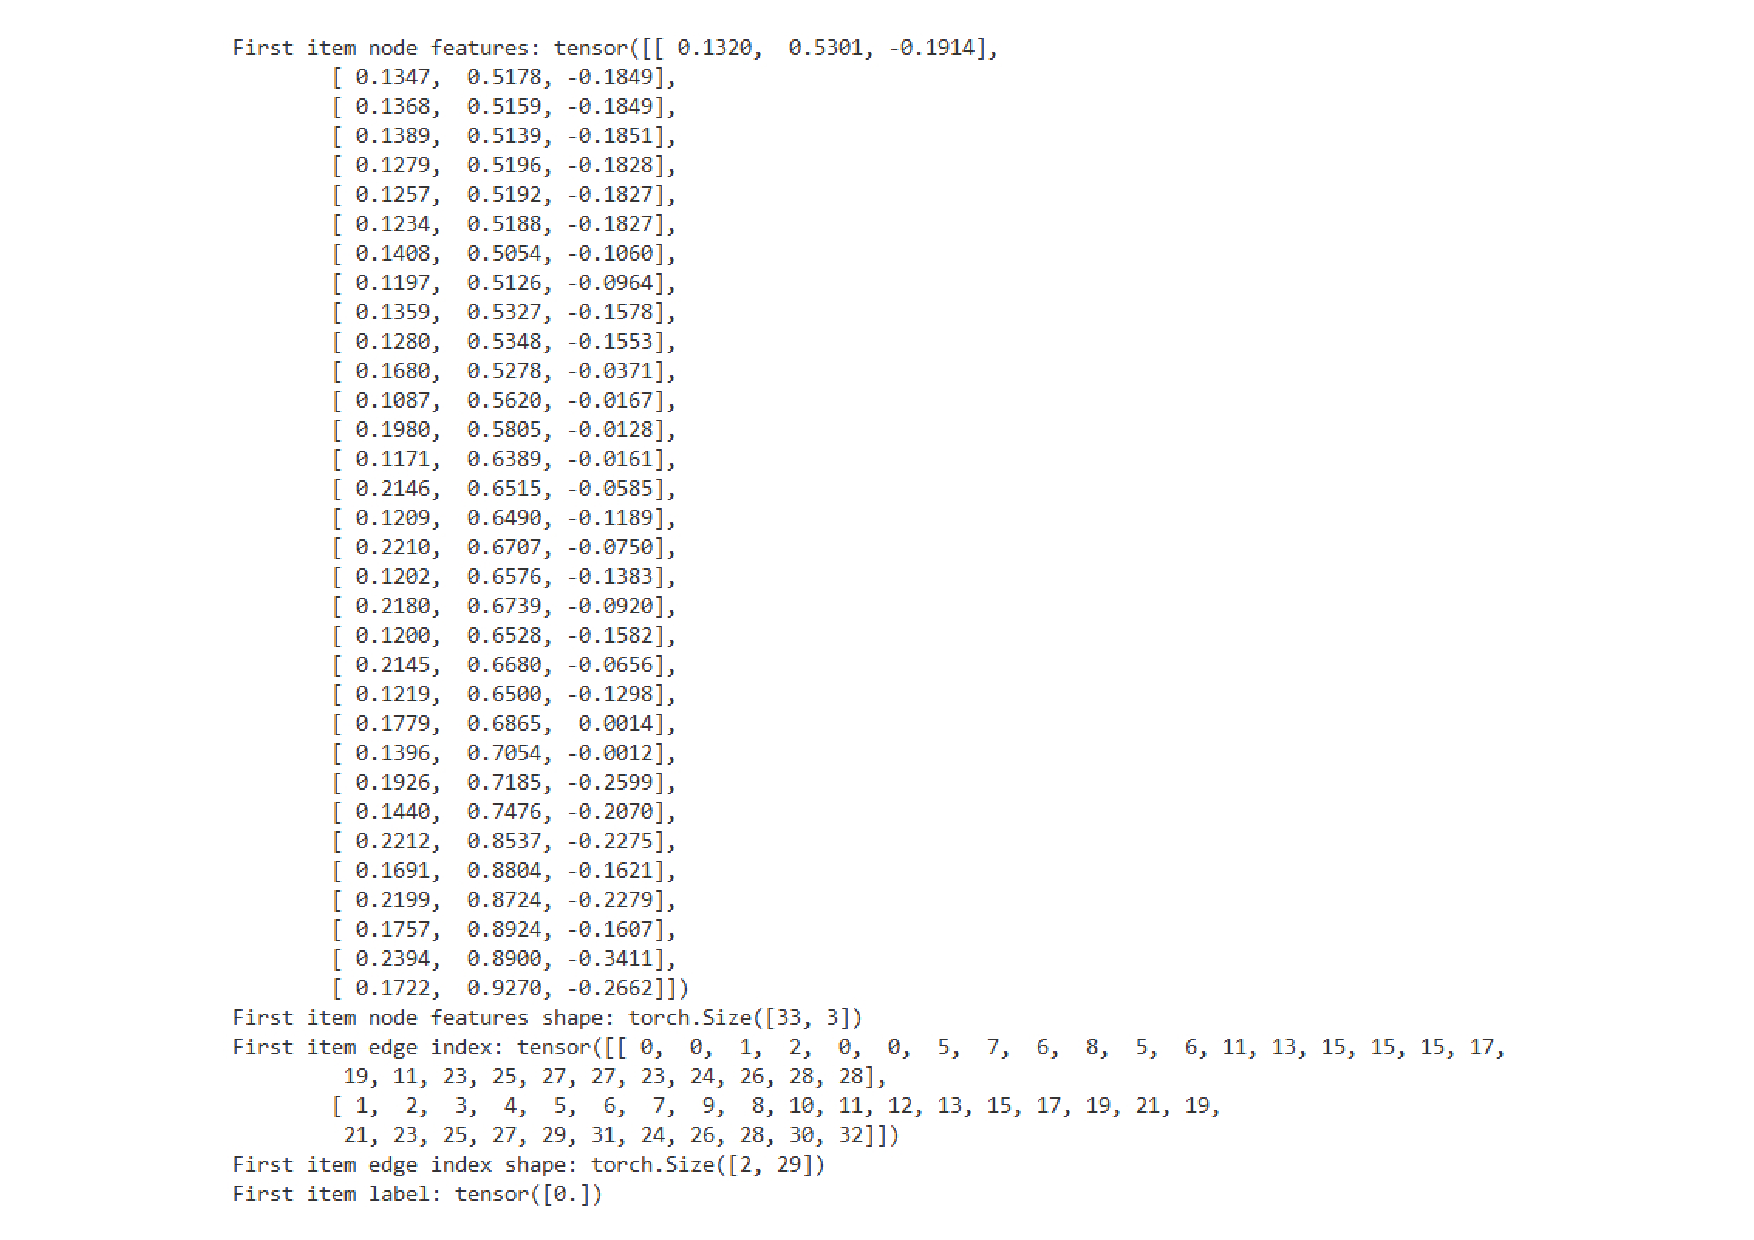
\includegraphics[width=0.9\textwidth]{figure/BAB 3/contoh data graf.pdf}
    \caption{Example of graph data representation}
    \label{fig:contoh data graf}
\end{figure}

\subsubsection{5-Fold Dataset Splitting}
\label{IV.K-Fold}

To prevent data leakage, the dataset was divided using folder-based 5-fold splitting rather than file-based splitting. One fold was used for validation and the remaining four folds were used for training in each iteration. Because folders contain different numbers of files, the number of training and validation samples varies across iterations.

\begin{table}[H]
    \centering
    \caption{Results of 5-fold dataset splitting by folder}
    \label{tab:data k-fold}
    \begin{tabular}{c c c c c c c c}
    \hline
    \multirow{2}{*}{\textbf{Iteration}} & \multicolumn{5}{c}{\textbf{Folders per Fold}} & \multirow{2}{*}{\textbf{Training Data}} & \multirow{2}{*}{\textbf{Validation Data}} \\ \cline{2-6}
     & \textbf{1} & \textbf{2} & \textbf{3} & \textbf{4} & \textbf{5} & & \\ \hline 
    1 & 100 & 100 & 100 & 100 & 99 & 6,969 & 2,531 \\ 
    2 & 100 & 100 & 100 & 100 & 99 & 8,151 & 1,349 \\ 
    3 & 100 & 100 & 100 & 100 & 99 & 7,159 & 2,341 \\ 
    4 & 100 & 100 & 100 & 100 & 99 & 7,922 & 1,578 \\ 
    5 & 100 & 100 & 100 & 100 & 99 & 7,799 & 1,701 \\ \hline
    \multicolumn{6}{c}{Total} & \multicolumn{2}{c}{9,500}\\ \hline
    \end{tabular}
\end{table}


\subsection{GCN Model Design}
\label{IV.Perancangan}

The proposed model, shown in Kode \ref{kode:inisialisasi gcn}, uses stacked GCNConv layers followed by BatchNorm1d, ReLU activation, and dropout. Residual connections are enabled when feature dimensions are compatible, helping gradient flow in deeper layers. After graph convolutions, global pooling aggregates node-level representations into graph-level embeddings, and a two-layer MLP performs binary classification with a sigmoid output. This design aims to capture spatial relations between body landmarks while maintaining stable training.

\subsection{Performance with Default Hyperparameters}
\label{IV.evaluasi-default}

The default training configuration is summarized in Table \ref{tab:hyperparams-gcn}. Training was conducted for 100 epochs with AdamW, a learning rate of \(1\times10^{-3}\), weight decay of \(1\times10^{-5}\), batch size 32, dropout 0.3, and hidden channels \([64, 32, 32, 32, 32]\).

\begin{table}[H]
    \centering
    \caption{Hyperparameter configuration for GCN training}
    \label{tab:hyperparams-gcn}
    \begin{tabular}{c c c}
        \hline
        \textbf{No} & \textbf{Hyperparameter} & \textbf{Value} \\ \hline
        1 & optimizers & AdamW \\ 
        2 & learning\_rates & 1e-3 \\ 
        3 & weight\_decays & 1e-5 \\ 
        4 & batch\_sizes & 32 \\ 
        5 & dropout\_rates & 0.3 \\ 
        6 & epochs & 100 \\ 
        7 & hidden\_channels & [64, 32, 32, 32, 32] \\ 
        8 & residuals & True \\ \hline
    \end{tabular}
\end{table}

The 5-fold results in Table \ref{tab:evaluasi-fold} show that the model achieved an average accuracy of 0.665, precision of 0.694, recall of 0.590, and F1-score of 0.638. The best fold was Fold 4, with accuracy 0.711 and F1-score 0.717. Overall, precision was consistently higher than recall, indicating that the model was more conservative and tended to reduce false positives at the expense of missing some fall cases.

\begin{table}[H]
    \centering
    \caption{Default configuration results for each fold and their average}
    \label{tab:evaluasi-fold}
    \begin{tabular}{c c c c c c c c c}
        \hline
        \multirow{2}{*}{\textbf{Fold}} & \multicolumn{4}{c}{\textbf{Confusion Matrix}} & \multicolumn{4}{c}{\textbf{Evaluation Metrics}} \\ \cline{2-9}
         & \textbf{TP} & \textbf{TN} & \textbf{FP} & \textbf{FN} & \textbf{Acc} & \textbf{Pre} & \textbf{Rec} & \textbf{F1} \\ \hline
        1 & 558 & 1105 & 592 & 276 & 0.657 & 0.696 & 0.657 & 0.667 \\ 
        2 & 613 & 232 & 43 & 461 & 0.626 & \textbf{0.812} & 0.626 & 0.662 \\ 
        3 & 425 & 1165 & 299 & 452 & 0.679 & 0.671 & 0.679 & 0.672 \\ 
        4 & 703 & 419 & 138 & 318 & \textbf{0.711} & 0.742 & \textbf{0.711} & \textbf{0.717} \\ 
        5 & 501 & 594 & 163 & 443 & 0.644 & 0.674 & 0.644 & 0.641 \\ \hline
        \multicolumn{5}{c}{Average} & 0.665 & 0.694 & 0.590 & 0.638 \\ \hline
    \end{tabular}
\end{table}

Figure \ref{fig:tren akurasi pelatihan default} shows the validation accuracy trend across epochs. The curve increases gradually from about 0.60--0.62 to around 0.68--0.69 and becomes relatively stable after approximately epoch 35--40. No strong sign of overfitting appears in the validation curve, suggesting that the default configuration provides stable learning.

\begin{figure}[H]
    \centering
    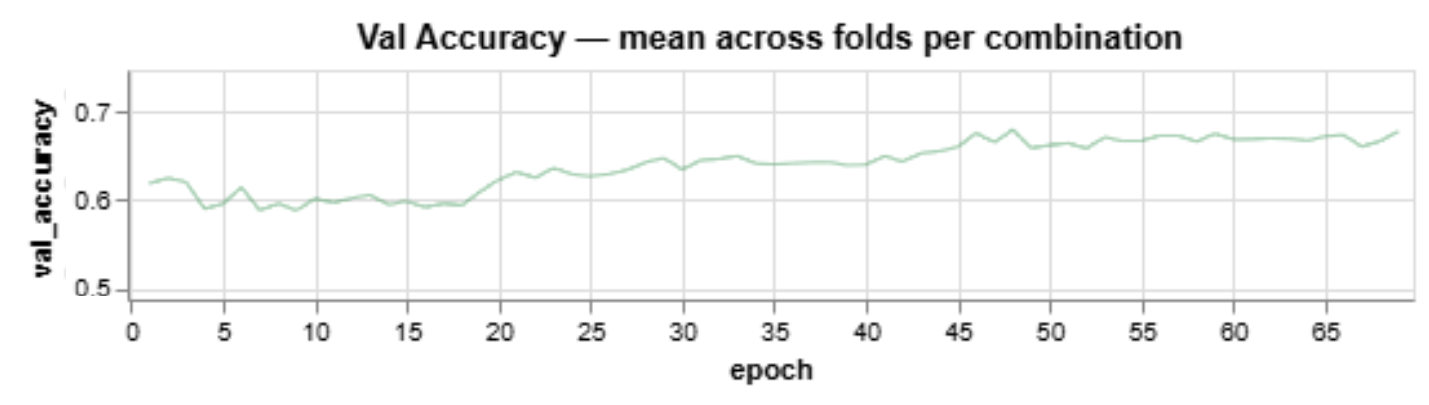
\includegraphics[width=0.8\textwidth]{figure/BAB 4/akurasi model hyperparameter default.png}
    \caption{Validation accuracy trend of GCN training with default hyperparameters}
    \label{fig:tren akurasi pelatihan default}
\end{figure}

\subsection{Primary Data Testing}
\label{IV.testing}

The best model weights were taken from Fold 4 at epoch 2, with validation accuracy 0.71, and then evaluated on primary data. Figure \ref{fig:cm testing} shows that the model correctly predicted 22 fall images, but it also frequently classified non-fall samples as fall.

\begin{figure}[H]
    \centering
    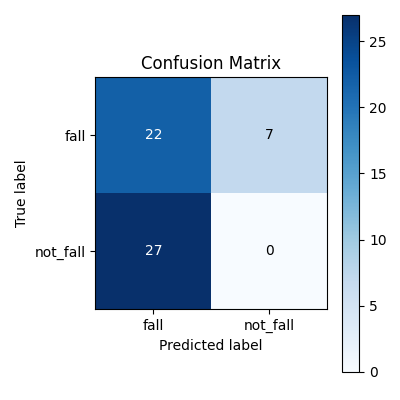
\includegraphics[width=0.55\textwidth]{figure/BAB 4/testing_confusion_matrix.png}
    \caption{Confusion matrix on primary test data}
    \label{fig:cm testing}
\end{figure}

Table \ref{tab:evaluasi-testing} shows that the test accuracy was only 0.39, with precision 0.45, recall 0.76, and F1-score 0.56. This weak performance indicates poor generalization to the primary data, especially for the non-fall class. A likely explanation is that the non-fall test set contains chair-sitting activities that are visually similar to fall transitions. In addition, the balancing stage may have reduced the representation of these transition patterns, making the model less robust on such cases.

\begin{table}[H]
\centering
\caption{Testing results on primary data}
\label{tab:evaluasi-testing}
\begin{tabular}{c c c c c c c c}
\hline
\multicolumn{4}{c}{\textbf{Confusion Matrix}} &
\multicolumn{4}{c}{\textbf{Evaluation Metrics}} \\
\hline
\textbf{TP} & \textbf{TN} & \textbf{FP} & \textbf{FN} &
\textbf{Acc} & \textbf{Pre} & \textbf{Rec} & \textbf{F1} \\
\hline
22 & 0 & 27 & 7 & 0.39 & 0.45 & 0.76 & 0.56 \\
\hline
\end{tabular}
\end{table}

% Examples of final predictions are presented in Table \ref{tab:prediksi_model}.

% \begin{table}[htbp]
% \centering
% \caption{Examples of final model predictions}
% \label{tab:prediksi_model}
% \begin{tabular}{|c|>{\centering\arraybackslash}p{0.35\textwidth}|>{\centering\arraybackslash}p{0.18\textwidth}|>{\centering\arraybackslash}p{0.18\textwidth}|}
% \hline
% \textbf{No} & \textbf{Input Image} & \textbf{Predicted Result} & \textbf{Actual Label} \\
% \hline
% 1 &
% 
\includegraphics[trim=0cm 0cm 0cm 18cm, clip, width=\linewidth,height=5.0cm,keepaspectratio]{images/fall/fall_1.jpg} &
% non-fall &
% fall \\
% \hline
% 2 &
% 
\includegraphics[trim=0cm 0cm 0cm 18cm, clip, width=\linewidth,height=5.0cm,keepaspectratio]{images/fall/fall_2.jpg} &
% fall &
% fall \\
% \hline
% 3 &
% 
\includegraphics[trim=0cm 0cm 0cm 18cm, clip, width=\linewidth,height=5.0cm,keepaspectratio]{images/fall/fall_3.jpg} &
% fall &
% fall \\
% \hline
% 4 &
% 
\includegraphics[trim=0cm 0cm 0cm 18cm, clip, width=\linewidth,height=5.0cm,keepaspectratio]{images/not_fall/not_fall_0.jpg} &
% fall &
% non-fall \\
% \hline
% 5 &
% 
\includegraphics[trim=0cm 0cm 0cm 18cm, clip, width=\linewidth,height=5.0cm,keepaspectratio]{images/not_fall/not_fall_1.jpg} &
% fall &
% non-fall \\
% \hline
% 6 &
% 
\includegraphics[trim=0cm 0cm 0cm 18cm, clip, width=\linewidth,height=5.0cm,keepaspectratio]{images/not_fall/not_fall_2.jpg} &
% fall &
% non-fall \\
% \hline
% \end{tabular}
% \end{table}

\subsection{Ablation Study}
\label{IV.evaluasi-ablasi}

The ablation study was conducted to examine the contribution of five hyperparameters: optimizer, learning rate, batch size, weight decay, and dropout. All experiments were performed on Fold 4 because the default configuration achieved its highest validation accuracy on this fold. In each experiment, one hyperparameter was varied while the others were kept constant.

\subsubsection{Optimizer}
\label{IV.optimizer}

RMSProp produced the best accuracy, recall, and F1-score among the tested optimizers. AdamW produced fewer false positives, while LION gave the weakest overall performance.

\begin{table}[H]
    \centering
    \caption{Ablation study results for optimizer}
    \label{tab:ablasi optimizer}
    \begin{tabular}{c c c c c c c c c}
        \hline
        \multirow{2}{*}{\textbf{Optimizer}} & \multicolumn{4}{c}{\textbf{Confusion Matrix}} & \multicolumn{4}{c}{\textbf{Evaluation Metrics}} \\ \cline{2-9}
         & \textbf{TP} & \textbf{TN} & \textbf{FP} & \textbf{FN} & \textbf{Acc} & \textbf{Pre} & \textbf{Rec} & \textbf{F1} \\ \hline
        AdamW & 1147 & 549 & 285 & 550 & 0.670 & 0.702 & 0.670 & 0.679 \\ 
        RMSProp & 1222 & 531 & 303 & 475 & \textbf{0.693} & 0.711 & 0.693 & 0.699 \\ 
        LION & 1158 & 523 & 311 & 539 & 0.664 & 0.691 & 0.664 & 0.672 \\ \hline
    \end{tabular}
\end{table}

\subsubsection{Learning Rate}
\label{IV.lr}

A learning rate of \(1\times10^{-2}\) yielded the strongest overall performance, with the highest TP and the lowest FN, although it also produced more FP. Lower learning rates made the model more conservative but reduced recall.

\begin{table}[H]
    \centering
    \caption{Ablation study results for learning rate}
    \label{tab:ablasi lr}
    \begin{tabular}{c c c c c c c c c}
        \hline
        \multirow{2}{*}{\textbf{Learning Rate}} & \multicolumn{4}{c}{\textbf{Confusion Matrix}} & \multicolumn{4}{c}{\textbf{Evaluation Metrics}} \\ \cline{2-9}
         & \textbf{TP} & \textbf{TN} & \textbf{FP} & \textbf{FN} & \textbf{Acc} & \textbf{Pre} & \textbf{Rec} & \textbf{F1} \\ \hline
        1e-2 & 1469 & 427 & 407 & 228 & \textbf{0.749} & 0.740 & 0.749 & 0.740 \\ 
        1e-3 & 1132 & 528 & 306 & 565 & 0.656 & 0.687 & 0.656 & 0.665 \\ 
        1e-4 & 1045 & 569 & 265 & 652 & 0.638 & 0.688 & 0.638 & 0.649 \\ \hline
    \end{tabular}
\end{table}

\subsubsection{Batch Size}
\label{IV.batch_size}

Batch size 64 showed the best accuracy and F1-score. Batch size 32 reduced false positives but also lowered recall and overall accuracy.

\begin{table}[H]
    \centering
    \caption{Ablation study results for batch size}
    \label{tab:ablasi batch size}
    \begin{tabular}{c c c c c c c c c}
        \hline
        \multirow{2}{*}{\textbf{Batch Size}} & \multicolumn{4}{c}{\textbf{Confusion Matrix}} & \multicolumn{4}{c}{\textbf{Evaluation Metrics}} \\ \cline{2-9}
         & \textbf{TP} & \textbf{TN} & \textbf{FP} & \textbf{FN} & \textbf{Acc} & \textbf{Pre} & \textbf{Rec} & \textbf{F1} \\ \hline
        16 & 1149 & 531 & 303 & 548 & 0.664 & 0.693 & 0.664 & 0.672 \\ 
        32 & 1105 & 560 & 274 & 592 & 0.658 & 0.697 & 0.658 & 0.668 \\ 
        64 & 1218 & 521 & 313 & 479 & \textbf{0.687} & 0.705 & 0.687 & 0.693 \\ \hline
    \end{tabular}
\end{table}

\subsubsection{Weight Decay}
\label{IV.weight-decay}

The best result was achieved with weight decay \(1\times10^{-6}\), which gave the most balanced trade-off between detection performance and false alarms.

\begin{table}[H]
    \centering
    \caption{Ablation study results for weight decay}
    \label{tab:ablasi Weight Decay}
    \begin{tabular}{c c c c c c c c c}
        \hline
        \multirow{2}{*}{\textbf{Weight Decay}} & \multicolumn{4}{c}{\textbf{Confusion Matrix}} & \multicolumn{4}{c}{\textbf{Evaluation Metrics}} \\ \cline{2-9}
         & \textbf{TP} & \textbf{TN} & \textbf{FP} & \textbf{FN} & \textbf{Acc} & \textbf{Pre} & \textbf{Rec} & \textbf{F1} \\ \hline
        1e-4 & 1300 & 508 & 326 & 397 & 0.714 & 0.721 & 0.714 & 0.717 \\ 
        1e-5 & 1344 & 483 & 351 & 353 & 0.722 & 0.722 & 0.722 & 0.722 \\ 
        1e-6 & 1321 & 511 & 323 & 376 & \textbf{0.724} & 0.729 & 0.724 & 0.726 \\ \hline
    \end{tabular}
\end{table}

\subsubsection{Dropout}
\label{IV.dropout}

Dropout 0.2 gave the highest accuracy and F1-score. Increasing dropout reduced false alarms slightly, but it also caused more fall cases to be missed.

\begin{table}[H]
    \centering
    \caption{Ablation study results for dropout}
    \label{tab:ablasi Dropout}
    \begin{tabular}{c c c c c c c c c}
        \hline
        \multirow{2}{*}{\textbf{Dropout}} & \multicolumn{4}{c}{\textbf{Confusion Matrix}} & \multicolumn{4}{c}{\textbf{Evaluation Metrics}} \\ \cline{2-9}
         & \textbf{TP} & \textbf{TN} & \textbf{FP} & \textbf{FN} & \textbf{Acc} & \textbf{Pre} & \textbf{Rec} & \textbf{F1} \\ \hline
        0.2 & 1178 & 557 & 277 & 519 & \textbf{0.686} & 0.713 & 0.686 & 0.693 \\ 
        0.3 & 1138 & 521 & 313 & 559 & 0.656 & 0.685 & 0.656 & 0.664 \\ 
        0.4 & 1102 & 559 & 275 & 595 & 0.656 & 0.696 & 0.656 & 0.666 \\ \hline
    \end{tabular}
\end{table}

\subsection{Comparison Between Default and Ablation Settings}
\label{IV.Analisis}

The best settings identified by the ablation study are summarized in Table \ref{tab:hyperparams-default-ablasi}. Compared with the default setting, the optimized configuration uses RMSProp, a higher learning rate, larger batch size, lower weight decay, and lower dropout.

\begin{table}[H]
    \centering
    \caption{Comparison between default hyperparameters and ablation results}
    \label{tab:hyperparams-default-ablasi}
    \begin{tabular}{c c c c}
        \hline
        \textbf{No} & \textbf{Hyperparameter} & \textbf{Default} & \textbf{Ablation Result} \\ \hline
        1 & optimizers & AdamW & RMSProp \\ 
        2 & learning rate & 1e-3 & 1e-2 \\ 
        3 & batch size & 32 & 64 \\ 
        4 & weight decay & 1e-5 & 1e-6 \\ 
        5 & dropout rate & 0.3 & 0.2 \\ 
        6 & hidden\_channels & [64, 32, 32, 32, 32] & [64, 32, 32, 32, 32] \\ 
        7 & epochs & 100 & 100 \\ 
        8 & residuals & True & True \\ \hline
    \end{tabular}
\end{table}

The 5-fold evaluation of the optimized configuration is shown in Table \ref{tab:evaluasi-fold-ablasi}. The average accuracy increased to 0.683, precision to 0.718, recall to 0.683, and F1-score to 0.687. The best fold was Fold 1, which achieved accuracy 0.725 and F1-score 0.723.

\begin{table}[H]
    \centering
    \caption{Ablation-based configuration results for each fold and their average}
    \label{tab:evaluasi-fold-ablasi}
    \begin{tabular}{c c c c c c c c c}
        \hline
        \multirow{2}{*}{\textbf{Fold}} & \multicolumn{4}{c}{\textbf{Confusion Matrix}} & \multicolumn{4}{c}{\textbf{Evaluation Metrics}} \\ \cline{2-9}
         & \textbf{TP} & \textbf{TN} & \textbf{FP} & \textbf{FN} & \textbf{Acc} & \textbf{Pre} & \textbf{Rec} & \textbf{F1} \\ \hline
        1 & 458 & 1378 & 319 & 376 & \textbf{0.725} & 0.721 & \textbf{0.725} & \textbf{0.723} \\ 
        2 & 677 & 216 & 59 & 397 & 0.662 & \textbf{0.804} & 0.662 & 0.695 \\ 
        3 & 410 & 1181 & 283 & 467 & 0.680 & 0.670 & 0.680 & 0.670 \\ 
        4 & 719 & 410 & 147 & 302 & 0.716 & 0.741 & 0.716 & 0.721 \\ 
        5 & 500 & 573 & 184 & 444 & 0.631 & 0.656 & 0.631 & 0.628 \\ \hline
        \multicolumn{5}{c}{Average} & 0.683 & 0.718 & 0.683 & 0.687 \\ \hline
    \end{tabular}
\end{table}

A direct comparison between the default and optimized settings is provided in Table \ref{tab:perbandingan cm default ablasi}. In general, the ablation-based configuration improves performance, although the improvement is not uniform across all folds. The clearest gain appears in the reduction of false alarms in several folds, especially through higher TN values. This suggests that the optimized configuration improves the model's stability in recognizing non-fall activities while still maintaining competitive fall detection.

\begin{table}[H]
    \centering
    \caption{Comparison of evaluation results per fold between default and ablation-based configurations}
    \label{tab:perbandingan cm default ablasi}
    \begin{tabular}{c c c c c c c c c c}
        \hline
        \multirow{2}{*}{\textbf{Fold}} & \multirow{2}{*}{\textbf{Configuration}} & \multicolumn{4}{c}{\textbf{Confusion Matrix}} & \multicolumn{4}{c}{\textbf{Evaluation Metrics}} \\ \cline{3-10}
         & & \textbf{TP} & \textbf{TN} & \textbf{FP} & \textbf{FN} & \textbf{Acc} & \textbf{Pre} & \textbf{Rec} & \textbf{F1} \\ \hline
        1 & Default & 558 & 1105 & 592 & 276 & 0.657 & 0.696 & 0.657 & 0.667 \\ 
          & Ablation & 458 & \textbf{1378} & 319 & 376 & \textbf{0.725} & 0.721 & \textbf{0.725} & \textbf{0.723} \\ 
        2 & Default & 613 & 232 & 43 & 461 & 0.626 & \textbf{0.812} & 0.626 & 0.662 \\ 
          & Ablation & 677 & 216 & 59 & 397 & 0.662 & 0.804 & 0.662 & 0.695 \\ 
        3 & Default & 425 & 1165 & 299 & 452 & 0.679 & 0.671 & 0.679 & 0.672 \\ 
          & Ablation & 410 & 1181 & 283 & 467 & 0.680 & 0.670 & 0.680 & 0.670 \\
        4 & Default & 703 & 419 & 138 & 318 & 0.711 & 0.742 & 0.711 & 0.717 \\ 
          & Ablation & \textbf{719} & 410 & 147 & 302 & 0.716 & 0.741 & 0.716 & 0.721 \\ 
        5 & Default & 501 & 594 & 163 & 443 & 0.644 & 0.674 & 0.644 & 0.641 \\ 
          & Ablation & 500 & 573 & 184 & 444 & 0.631 & 0.656 & 0.631 & 0.628 \\ \hline
    \end{tabular}
\end{table}

The average metric comparison in Table \ref{tab:perbandingan hasil hyperparameter default dan studi ablasi} confirms that the ablation-based configuration outperformed the default configuration. Accuracy increased by 0.018, precision by 0.024, recall by 0.093, and F1-score by 0.049. The largest gain was observed in recall, which indicates that the optimized setting reduced missed fall cases more effectively.

\begin{table}[H]
    \centering
    \caption{Average evaluation comparison between default and ablation-based configurations}
    \label{tab:perbandingan hasil hyperparameter default dan studi ablasi}
    \begin{tabular}{c c c c c}
        \hline
        \multirow{2}{*}{\textbf{Hyperparameter Configuration}} & \multicolumn{4}{c}{\textbf{Average Evaluation Metrics}} \\ \cline{2-5}
         & \textbf{Acc} & \textbf{Pre} & \textbf{Rec} & \textbf{F1} \\ \hline
        Default & 0.665 & 0.694 & 0.590 & 0.638 \\ 
        Ablation Study & \textbf{0.683} & \textbf{0.718} & \textbf{0.683} & \textbf{0.687} \\ \hline
    \end{tabular}
\end{table}

Although the ablation-based configuration improved the proposed model, its performance remained below that reported by Zhang et al. (2023), who achieved 96.3\% accuracy on the MCF dataset \cite{Zhang2023}. This gap is reasonable because Zhang et al. used a Dense Spatial-Temporal Graph Convolutional Network, which explicitly models both spatial and temporal dependencies across consecutive frames. In contrast, this study intentionally used a simpler GCN architecture without explicit spatio-temporal modeling and relied only on skeleton features extracted by MediaPipe Pose. Therefore, the lower performance in this work reflects the architectural limitation of the simpler model, while also showing that a basic skeleton-based GCN can still provide meaningful discrimination between fall and non-fall classes.


\section{CONCLUSION}
\label{}

This study achieved its main objective of developing an end-to-end fall detection pipeline based on human pose landmarks and Graph Convolutional Networks (GCN). The proposed framework starts from video frame extraction, continues with pose estimation using MediaPipe Pose to obtain 33 body landmarks, and transforms the landmark coordinates into graph-structured data with skeleton edges for binary fall/non-fall classification. To ensure a reliable evaluation, the dataset was divided using 5-fold cross-validation based on group or folder prefix, which prevented data leakage between training and validation sets.

The experimental results show that the default model configuration produced an average accuracy of 0.665, precision of 0.694, recall of 0.590, and F1-score of 0.638, indicating that the model was relatively good at reducing false positives but still missed some fall events. Furthermore, the ablation study demonstrated that several hyperparameter adjustments, namely RMSProp optimizer, learning rate of $1\times10^{-2}$, batch size of 64, weight decay of $1\times10^{-6}$, and dropout of 0.2, improved the model performance. With this configuration, the average accuracy increased to 0.683, precision to 0.718, recall to 0.683, and F1-score to 0.687. These results confirm that hyperparameter selection has a meaningful effect on the effectiveness of pose-based fall detection.

Overall, the findings indicate that the proposed method is feasible for representing spatial pose dynamics and classifying fall events. Although the performance improvement is still moderate, the optimized configuration is more reliable than the default setting for this task. Future research may extend this work by incorporating temporal graph modeling, larger and more diverse datasets, multimodal features, or real-time deployment scenarios to improve robustness and support practical fall detection applications.

\section{ACKNOWLEDGEMENTS}
\label{}
The authors would like to thank Mr. Martin Clinton Tosima Manullang, Ph.D. and Ms. Leslie Anggraini, S.Kom., M.Cs. for constructive guidance and valuable suggestions throughout the study.

\section{DECLARATIONS}
\label{}
AUTHOR CONTIBUTION\\
Author 1 conducted the study, collected and analyzed the data,developed the project and prepared the manuscript. Author 2 and Author 3 supervised the research process and provided critical revisions to the manuscript. All authors approved the final version of the manuscript.

FUNDING STATEMENT\\
This research received no external funding.

COMPETING INTEREST \\
The authors declare no conflict of interest in this article.


\bibliographystyle{IEEEtran}
%jika ingin pakai mendeley aktifkan perintah dibawah ini 
\bibliography{refferences}
%aktifkan perintah dibawah ini jika artikel berakhir pada halaman GANJIL
%\newpage
%\begin{center}
%	\textbf{[This page intentionally left blank.]}
%\end{center}
\end{document}

%%
%% Akhir dari file `Matrik English.tex'. 